\documentclass[12pt,a4paper]{article}
\usepackage{a4wide}

% Fond encoding
\usepackage[T1]{fontenc}

% Lots of packpages
\usepackage[show]{ed}
\usepackage{enumitem}
\usepackage{hyperref}
\usepackage{pdfpages}
\usepackage{amstext,amssymb}
\usepackage{xspace}

% Tables and stuff
\usepackage{tabularx}
\usepackage{multirow}

\usepackage{wrapfig}
\usepackage[section]{placeins}
\usepackage{graphicx}
\usepackage{subcaption}

% For examples
\usepackage{amsthm}

% Example environment
\theoremstyle{remark}
\newtheorem{example}{Example}

% Examples = Tables = Figures
\makeatletter
\let\c@example\c@figure
\let\c@table\c@figure
\makeatother
\renewcommand{\thefigure}{\arabic{example}}
\renewcommand{\thetable}{\arabic{example}}

% tikz for mmt things
\usepackage{tikz}
\def\thmo#1#2{\mathsf{#1}\colon\kern-.15em{#2}}% for theories
\usetikzlibrary{shapes,arrows,mmt,fit,shadows}

% Copyright and Stuff
\usepackage[
    type={CC},
    modifier={by-sa},
    version={4.0},
]{doclicense}

\providecommand{\inlinecode}[1]{{\lstinline[language=qmt]|#1|}}

\providecommand{\identifier}[1]{%
  \StrSubstitute{#1}{\_}{_}[\identifiertmp]
  \expandafter\path\expandafter{\identifiertmp}%
}
\let\uri\identifier% \uri and \idenfitier are the same
\def\meta#1{\ensuremath{\langle\kern-.25em\langle}#1\ensuremath{\rangle\kern-.2em\rangle}}

% abbreviations
\providecommand{\mmt}{MMT}
\providecommand{\omdocmmt}{OMDoc/MMT}
\providecommand{\lmfdb}{LMFDB}

% More abbreviatons for diagrams and things
\def\plaintt#1{\ifmmode\mathrm{\texttt{#1}}\else\texttt{#1}\fi}
\def\typett{\plaintt{type}}
\def\codectt{\plaintt{codec}}

% colors for syntax highlighting
\usepackage{xcolor}
\colorlet{punct}{red!60!black}
\definecolor{background}{HTML}{EEEEEE}
\definecolor{delim}{RGB}{20,105,176}
\colorlet{numb}{magenta!60!black}

% Syntax hightlighting
\usepackage{listings}

% JSON syntax
\lstdefinelanguage{json}{
    basicstyle=\footnotesize\sffamily,
    numberstyle=\scriptsize,
    showstringspaces=false,
    breaklines=true,
    frame=single, 
    literate=
     *{0}{{{\color{numb}0}}}{1}
      {1}{{{\color{numb}1}}}{1}
      {2}{{{\color{numb}2}}}{1}
      {3}{{{\color{numb}3}}}{1}
      {4}{{{\color{numb}4}}}{1}
      {5}{{{\color{numb}5}}}{1}
      {6}{{{\color{numb}6}}}{1}
      {7}{{{\color{numb}7}}}{1}
      {8}{{{\color{numb}8}}}{1}
      {9}{{{\color{numb}9}}}{1}
      {:}{{{\color{punct}{:}}}}{1}
      {,}{{{\color{punct}{,}}}}{1}
      {\{}{{{\color{delim}{\{}}}}{1}
      {\}}{{{\color{delim}{\}}}}}{1}
      {[}{{{\color{delim}{[}}}}{1}
      {]}{{{\color{delim}{]}}}}{1},
}

% The Scala language
\lstdefinelanguage{scala}{
  basicstyle=\footnotesize\ttfamily,
  breaklines=true,
  morekeywords={abstract,case,catch,class,def,%
    do,else,extends,false,final,finally,%
    for,if,implicit,import,match,mixin,%
    new,null,object,override,package,%
    private,protected,requires,return,sealed,%
    super,this,throw,trait,true,try,%
    type,val,var,while,with,yield},
  otherkeywords={=>,<-,<\%,<:,>:,\#,@},
  sensitive=true,
  morecomment=[l]{//},
  morecomment=[n]{/*}{*/},
  morestring=[b]",
  morestring=[b]',
  morestring=[b]"""
}

% XML is fun
\lstdefinelanguage{XML}
{
  basicstyle=\footnotesize\ttfamily,
  showstringspaces=false,
  breaklines=true,
  morestring=[b]",
  morestring=[s]{>}{<},
  morecomment=[s]{<?}{?>},
  morekeywords={}% list your attributes here
}

% for QMT queries
\lstdefinelanguage{qmt}{
    basicstyle=\footnotesize\ttfamily,
    showstringspaces=false,
    frame=single, 
    mathescape, 
    columns=fullflexible,
    breaklines=true
}

\setcounter{secnumdepth}{2}

% needs the KWARC bibliography setup, see
% https://github.com/KWARC/bibs
\usepackage[maxbibnames=99,style=alphabetic]{biblatex}
\addbibresource{kwarc.bib}


% Meta-data
\title{Enabling Cross-System Communication Using Virtual Theories and QMT}
\author{Tom Wiesing}

\date{August 15, 2017}

\begin{document}
  % Template for Jacobs Master Thesis Title Page
\makeatletter
\begin{titlepage}
  \thispagestyle{empty}
  
  \providecommand{\HRule}{\vspace{-0.3cm}\rule{.45\linewidth}{0.5mm}}
  \providecommand{\printreviewer}[1]{
    \HRule\\
    \vspace*{-0.4em}
    {\small{#1}}\\[1ex]
  }
  
  
  % The university logo
  \vspace*{-3cm}
  \hfill 
\includegraphics[width=0.5\textwidth]{imgs/jacobs} \\[1cm]
  \vspace*{7mm}  
  
  % Title and Things
  \begin{center}
    \LARGE {
      \textbf{\@title}\\
      \bigskip
      by\\
      \bigskip
      \textbf{\@author\space}
    }
  \end{center}
  
  
  \vspace*{2.1cm}
  {
    \hspace*{-0.6cm}
    \centerline{
      \large{a thesis for conferral of a Master of Science in Data Engineering}
    }
  }

  \vfill
  
  % List of reviewers
  \Large{
    \begin{flushright}
      \printreviewer{Prof. Dr. Michael Kohlhase}
      \printreviewer{Dr. Florian Rabe}
    \end{flushright}
  }
  
  \vspace{1.5cm}
  
  % Date of Submission
  \begin{flushleft}
    \small{Date Of Submission: {\makeatletter\@date\makeatother}}\\
    \vspace{-0.4cm}
    ~\hrule
  \end{flushleft}
  
\end{titlepage}
\newpage

  % Template for Jacobs Master Thesis Declaration Page
\thispagestyle{empty}

\vspace*{\fill}

\begin{center}
  \LARGE {
    \textbf{Statutory Declaration}
  }
\end{center}

\vspace*{\baselineskip}

{
  \noindent
  I, {\makeatletter\@author\makeatother}, hereby declare that I have written this thesis independently, unless where clearly stated otherwise. 
  I have used only the sources, the data and the support that I have clearly mentioned. 
  This thesis has not been submitted for conferral of degree elsewhere.
}

\vspace*{\baselineskip}
\vspace*{\baselineskip}
\vspace*{\baselineskip}
\vspace*{\baselineskip}
\vspace*{\baselineskip}

{
  \noindent Bremen, {\makeatletter\@date\makeatother}
}

\vspace*{\baselineskip}
\vspace*{\baselineskip}
\vspace*{\baselineskip}
\vspace*{\baselineskip}

% Notice that this requires a signature scan and the margins need to be optimised per signature. 
% To create a signature, (1) scan it, (2) crop it into a pdf to create an appropriate .png file. 
% (3) use convert yoursignature.png yoursignature.bmp to create a bitmap, (3) use
% potrace yoursignature.bmp --eps to convert it to an eps file. If you signature looks
% bad (missing parts), try tweaking -k parameter of potrace with values between 0.5 and 1.0. 
%\makebox[0pt][l]{\hspace*{4cm}\raisebox{-5ex}{\includegraphics[height=5\baselineskip]{requirements/signature}}}%
\noindent Signature \hrulefill

\vspace*{\fill}

% and clear the page counter
\clearpage
\setcounter{page}{1}

\newpage


  
  \begin{abstract}
    Mathematical Knowledge Systems (MKS) are software solutions used by mathematicians in practice to explore specific fields of mathematics and help solving both abstract and computational problems. 
    To solve a specific problem multiple systems are often necessary. 
    
    Existing cross-system-communication solutions are ad-hoc, non-expandable, exist only for the most common system combinations and do not maintain semantics across systems. 
    Mathematicians are not interested in technical details required to use these approaches -- they only want to explore mathematics and solve problems. 
    In this thesis, we aim to address this problem by designing, implementing and demonstrating a generic, efficient and scalable approach for enabling transparent, semantics-aware, distributed computation across MKS. 
    
    \mmt\ is a language and framework that developed to manage mathematical knowledge. 
    It makes use of the theory graph metaphor by organizing knowledge within different concrete theories that are represented by files on disk. 
    To access knowledge in \mmt, users can make use a Query Language called QMT.
    
    In the OpenDreamKit project, an EU Horizon 2020 project aiming to provide tools for combining different existing mathematical software systems, we in particular want to make knowledge of these systems available to each other. 
    For this we make use of the so-called Math-In-The-Middle (MiTM) paradigm, a new mathematics-aware, semantic, extensible approach to connecting multiple systems. 
    Instead of building translations between any two of the involved systems, we decided to model the underlying mathematics in \mmt\ and only build interfaces between this Math-In-The-Middle and the systems. 
    
    On top of the MiTM approach, the concept of virtual theories is introduced to \mmt. 
    These are just like concrete theories, but without the assumption of loading all declarations from a file on disk at system startup. 
    We use them to transparently access knowledge across systems. 
    Additionally, we expand the QMT Query Language to enable mathematicians to send queries in a system-independent manner. 

    In this thesis, we first recap the existing architecture, then move on to discuss our implementation of the Math-In-The-Middle Approach. 
    Next we focus on the example of \lmfdb, a mathematical database of objects in number theory and show how it can be implemented as a Virtual Theory to enable the desired communication and computation. 
    Finally, we demonstrate the validity of our approach based on a concrete example. 
  \end{abstract}
\newpage

\tableofcontents

\vspace{\fill}\noindent
\doclicenseThis

\newpage
%\part{Introduction \& Preliminaries}
% !TEX root = ../thesis.tex
\section{Introduction}\label{sec:intro}

There are a multitude of different mathematical knowledge systems and tools. 
A mathematical knowledge system, or MKS, can be defined as a software solution which is aware of (a subset of) mathematical knowledge and can help mathematicians explore a specific field of mathematics. 

These systems can range from calculators, which are only capable of performing simple computations, via mathematical databases (storing a set of a mathematical objects) to powerful modeling tools and computer algebra systems (CAS), that feature a broad variety of features.
A few examples of common MKS include the databases like \cite{oeis} and \cite{lmfdb}, systems like \cite{gap} and \cite{sagemath}, or the Wolfram Mathematica \cite{mathematica11} Computer Algebra System. 

Most of these systems are very specific -- they focus on one or very few aspects of mathematics. 
For example, OEIS is a database of integer sequences and nothing else, 
LMFDB is a database of objects in number theory. 
GAP excels at discrete algebra, whereas SageMath focuses on Algebra and Geometry in general. 

For a mathematician however (a user; let us call her Jane) the systems themselves are not relevant, instead she only cares about being able to solve problems. 
Typically, it is not possible to solve a mathematical problem using only a single problem. 
Thus Jane needs to work with multiple systems and combine the results to reach a solution. 
Currently there is very little help with this practice, so Jane has to isolate sub-problems the respective systems are amenable to, formulate them into the respective input language, collect results, and reformulate them for the next system — a tedious and error-prone process at best, a significant impediment to scientific progress in its overall effect. 
Solutions for some situations certainly exist, which can help get Jane unstuck, but these are ad-hoc and for specific, often-used system combinations only. 
Each of these requires a lot of maintenance and does not scale to a larger set of specialist systems. 

In this thesis, we develop tools and methods of making mathematical software systems interoperable and contribute to a systematic, knowledge-based paradigm for system interoperability -- the \textbf{Math-in-the-Middle (MitM) paradigm} developed in the OpenDreamKit project -- a large-scale project that aims at providing a virtual research environment toolkit for mathematics based on existing (specialist) mathematical software systems. 

In the rest of the introduction, we will briefly review the concepts of the MitM paradigm leading to our research question before we embark in the technical discussion. 

\subsection{The MMT System, Libraries and MathHub}\label{sec:intro:mmt}

The center of the MitM paradigm is the \textbf{Math-in-the-Middle ontology}, a flexiformal representation of mathematical knowledge, which is represented in the the \omdocmmt language, mechanized by the MMT system, and stored in the MathHub information system. 

\mmt\ \cite{Rabe:MMTLanguageSystem09} is a language and framework that was developed to manage (mainly) mathematical knowledge. 
It can handle both formal and informal content. 
\mmt\ is under active development and the project home page can be found at \cite{uniformal:on}. 

Knowledge inside of \mmt\ employs the theory graph paradigm supported by the underlying \omdocmmt\ language. 
This means that knowledge is organized in distinct theories which are related by different relations in a graph-like manner. 
One of these relations is a so-called view, which can be used to translate knowledge from one theory to another. 
Definiens within each theory are identified by a URI (the so-called \mmt\ URI) whereas the definitions are represented by what amounts to OpenMath \cite{BusCapCar:oms04} objects. 
Apart from making purely formal declarations, it is also possible to annotate the declarations with human-readable, narrative elements. 

Commonly all knowledge in \mmt\ is manifested on disk and loaded by the system in its entirety on startup. 
This means that there is a set of files, specifically XML files, on disk containing the appropriate theories and declarations. 
We refer to theories stored in this form as \textit{concrete theories}. 

Knowledge in \mmt can be accessed by either giving it's name -- i.e. it's \mmt\ URI, 
or by giving a set of conditions that has to fulfilled by the knowledge in question. 
The achieve the latter, \mmt has a Query Language called QMT, which allows even complex conditions to be specified. 

This modeling of mathematical knowledge has proven very effective. 
On top of pure mathematical knowledge modeling, it is also possible to annotate declarations. 
This means one can give them human-readable descriptions.
The other direction, giving informal knowledge (for example a paper) a partially formal meaning is also possible.

This has allowed us to develop and populate a system called MathHub \cite{MathHub:on}. 
The system altogether forms a big theory graph totaling at about 10000 theories. 
MathHub is far more than just a theory graph however, it allows creating and editing of existing libraries and offers possibilities for integrating semantic services.
The deatils of this are not relevant to the topic at hand -- we refer the interested reader to \cite{Iancu:phd} instead.

Notable projects available on MathHub include SMGloM \cite{SMGloM:on} -- a semantic glossary of mathematical knowledge -- LATIN \cite{LATIN:online} -- a logical atlas of several different formalizations  -- as well as parts of the PVS \cite{PVSlibraries:on}, MiZar \cite{mizar:online} and HOL Light \cite{KalRab:hollight:14} libraries.

\subsection{Existing Ad-Hoc Solutions for System Interaction}\label{sec:intro:interact}

With the exception of Mathematica none of the previously mentioned systems attempt to be universal -- they do not try to model mathematics as a whole. 
Their focus on specific topics enables them to make concrete optimizations and provide detailed implementations of specific solutions. 

As a result, these systems work very differently -- for example databases only contain a fixed set of objects whereas computer algebra systems commonly allow for complicated manipulation of complex objects. 
This initially limits the inter actability of these systems, and makes it difficult for them to work together. 
Nonetheless, ad-hoc solutions exist and we proceed by giving the reader a brief overview. 

The situation is best illustrated by an example. 
Consider again our user Jane. 
She wishes to check the hypothesis that all abelian transitive groups are cyclic.
How can she go about verifying this hypothesis experimentally with the help of different MKS?

Jane realizes that the \lmfdb\ database contains a set of known abelian transitive groups. 
Furthermore, she realizes that the GAP system can check if a given group is cyclic. 
To check her hypothesis, she could first retrieve all relevant groups from \lmfdb, and then use GAP to check if each of these is cyclic. 
While a positive result would not formally prove her claim, it would certainly give her experimental evidence and show that she should try to prove this formally. 

% !TEX root = ../thesis.tex
\begin{wrapfigure}{r}{0.25\textwidth}
  \begin{center}
    \begin{tikzpicture}
      \node[draw] (a) at (0,.3) {A};
      \node[draw] (b) at (1,.3) {B};
      \node[draw] (c) at (1.7,1) {C};
      \node[draw] (d) at (1.7,2) {D};
      \node[draw] (e) at (1,2.7) {E};
      \node[draw] (f) at (0,2.7) {F};
      \node[draw] (g) at (-.7,2) {G};
      \node[draw] (h) at (-.7,1) {H};
      \draw (a) -- (b) -- (c) -- (d) -- (e) -- (f) -- (g) -- (h) -- (a);
      \draw (a) -- (c) -- (h) -- (d) -- (g) -- (e);
      \draw (b) -- (h);
      \draw (b) -- (f);
      \draw (b) -- (d);
      \draw (b) -- (g);
      \draw (b) -- (e);
      \draw (h) -- (e);
      \draw (d) -- (f);
      \draw (g) -- (c);
      \draw (a) -- (d);
      \draw (a) -- (e);
      \draw (a) -- (f);
      \draw (a) -- (g);
      \draw (e) -- (c);
      \draw (c) -- (f);
    \end{tikzpicture}
  \end{center}

  \caption[Classical Approach to connecting systems]{
    Common Ad-Hoc Approach to Connecting Systems. 
  }
  \label{fig:classicalconnect}
\end{wrapfigure}
How is such cross-system communication achieved in practice?
\lmfdb\ has implemented an export functionality of the database. 
Each time new data is available in \lmfdb\ it is exported and included in the SageMath software distribution. 
Within SageMath, Jane is provided with a low-level API that can then be used to access this dump. 

To communicate with GAP, a similar approach is chosen. 
A version of GAP is included within Sage, providing a GAP prompt. 
Again, Jane is provided with an interface to make use of GAP commands from within Sage. 

Jane has to first use the \lmfdb\ interface to find all abelian transitive groups. 
This means figuring out how \lmfdb\ works and then manually transferring the objects from \lmfdb\ to Sage. 
Next, she has to make sure that these objects are in a representation that GAP can understand. 
After some translation work, she can then open the GAP prompt in Sage and check for each group if GAP thinks it is cyclic. 

This is obviously a very tedious approach that can easily lead to mistakes. 
It also suffers from many other problems. 
\begin{description}
  \item[Semantic-less interfaces]
  When stating that \lmfdb\ it is exported and included in the SageMath software distribution describes the level of integration well. 
  The semantics of \lmfdb\ are not maintained during this process. 
  
  For example, boolean values are commonly represented as integers $1$ or $0$ in \lmfdb. 
  When accessing the same value from SageMath, no conversion into a SageMath boolean (which is in fact just a python object) is performed -- Jane still only sees a $1$ or a $0$. 
  The difference between $1$ and \inlinecode{true} may seem trivial, but this becomes an issue when talking about data types like matrices or vectors. 
  Continuing, Jane needs to know that the \inlinecode{ab} of a group object in \lmfdb\ is $1$ if it is abelian and $0$ if it is not. 
  
  This is not very mathematical, and it requires being familiar with the technical details of how groups are represented inside of \lmfdb. 

  \item[Updating Problem]
  This obviously requires packaging both \lmfdb\ and GAP for usage within Sage. 
  Each time a change is made in either of these systems, they need to be re-packaged and Sage needs to be updated. 
  This gives rise to a version management problem -- the usage of the newest versions of \lmfdb\ or GAP is not automatic --
  and a data duplication issue. 

  \item[Scaling Up]
  How is more complex communication managed?
  
  Imagine a user in GAP suddenly wanting to make use of \lmfdb. 
  This would mean having to add \lmfdb\ to GAP as well. 
  This not only means more data duplication, it also means having to build another bridge between two systems. 
  In general, to enable communication between $n$ systems each pair of systems need to be connected. 
  This means $O(n^2)$ connections need to be built, leading to a situation as in Figure~\ref{fig:classicalconnect}. 
\end{description}

Mathematica, unlike the other systems mentioned here, attempts to be a universal system. 
One one hand this does have the advantage that it can handle a large subset of Mathematics at once. 
On the other hand, by nature of being a commercial product and not an OpenSource effort, it is not entirely clear how interactions between different components are achieved. 
Mathematica is usually not able to connect to other software systems and mathematicians using Mathematica are required to use only tools available natively in the system. 

\subsection{The Math-In-The-Middle Approach}\label{sec:intro:mitm}

Recall that the OpenDreamKit \cite{OpenDreamKit:on} project is an EU-funded project that aims to create Virtual Research Environments enabling mathematicians to make efficient use of existing Open-Source mathematical knowledge systems. 
These systems include the aforementioned Sage, GAP and \lmfdb\ systems, along with others. 

We give a short overview of the OpenDreamKit project and involved systems here. 
For a a comprehensive list of all projects included in the OpenDreamKit project and in particular the Math-In-The-Middle approach we refer the interested reader to the OpenDreamKit project proposal \cite{ODKproposal:on} as well as reports on the Math-In-The-Middle approach \cite{DehKohKon:iop16}.

% !TEX root = ../thesis.tex
\begin{wrapfigure}{l}{0.3\textwidth}
  \begin{center}
    \begin{tikzpicture}[xscale=1.3,yscale=1.3]\normalsize
      \tikzstyle{withshadow}=[draw,drop shadow={opacity=.5},fill=white]
      \tikzstyle{system}=[draw]
      \tikzstyle{standard}=[circle,fill=blue!30]
      \tikzstyle{interface}=[circle,fill=purple!30,inner sep = 1pt,]
      \node[system] (a) at (0,.3) {A};
      \node[system] (b) at (1,.3) {B};
      \node[system] (c) at (1.7,1) {C};
      \node[system] (d) at (1.7,2) {D};
      \node[system] (e) at (1,2.7) {E};
      \node[system] (f) at (0,2.7) {F};
      \node[system] (g) at (-.7,2) {G};
      \node[system] (h) at (-.7,1) {H};
      \node[standard] (m) at (.5,1.5) {S};
      \node[interface] (ia) at (0.2,.9) {a};
      \node[interface] (ib) at (.8,.9) {b};
      \node[interface] (ic) at (1.1,1.2) {c};
      \node[interface] (id) at (1.1,1.75) {d};
      \node[interface] (ie) at (.8,2.1) {e};
      \node[interface] (if) at (0.2,2.1) {f};
      \node[interface] (ig) at (-.1,1.75) {g};
      \node[interface] (ih) at (-.1,1.2) {h};
      \draw (m) -- (ia) -- (a);
      \draw (m) -- (ib) -- (b);
      \draw (m) -- (ic) -- (c);
      \draw (m) -- (id) -- (d);
      \draw (m) -- (ie) -- (e);
      \draw (m) -- (if) -- (f);
      \draw (m) -- (ig) -- (g);
      \draw (m) -- (ih) -- (h);
      \end{tikzpicture}
  \end{center}

  \caption[The MITM Approach to Connecting Systems]{
    The MiTM Approach to Connecting Systems. 
  }
  \label{fig:mitmconnect}
\end{wrapfigure}
For this thesis, we build on and make use of the Math-In-The-Middle approach, which can be seen in Figure~\ref{fig:mitmconnect}. 
It models the true, underlying mathematical semantics in \mmt\ (blue $S$) and allows translation between this centrally formalized knowledge and the systems on the boundary (capital letters $A$ - $H$).
This mathematical knowledge is modeled using the well-established theory graph paradigm and is stored inside our MathHub / \mmt\ architecture. 

The knowledge in the systems themselves is also modeled via theories in a theory graph (small letters $a$ - $h$).
This allows us to implement translation with the help of bi-views -- views in both directions -- between the central knowledge -- the Math-In-The-Middle -- and each of the systems. 

Using this mechanism leaves the semantics of translated objects intact -- thus solving the first of the disadvantages listed above. 
Furthermore, when adding a new system it is only required to add $2$ new translations, one from the central math ontology to the system and one in the other direction. 
This drastically reduces the scaling problem -- suddenly only $O(n)$ translations are needed when connecting $n$ different systems. 

\subsection{Research Question}\label{sec:intro:rq}

This leads to our research question. 
How can different mathematical knowledge systems be connected in a generic, efficient and scalable manner to enable transparent, semantics-aware, distributed computation?

As we have seen, to solve this question and be semantics-aware it is required to model mathematics independent of the different systems. 
We need to separate the representations of objects inside each of the systems from their mathematical meaning, the semantics. 
This is achieved by using the semantics-aware, scaleable Math-In-The-Middle approach. 

However, the Math-In-The-Middle approach only provides part of the answer to this question. 
A complete solution needs to address three more aspects which are:
\begin{enumerate}[label={(\roman*)}]
  \item \label{intro:rq:vt} a generic mechanism to manage knowledge stored in the systems and keep it in sync with the Math-In-The-Middle ontologies, 
  \item \label{intro:rq:ql} a system-independent query language, capable of allowing users like Jane to transparently formulate computational problems to be solved, and
  \item \label{intro:rq:com} an efficient lower-level communication layer capable of transporting computational tasks and results between systems, allowing the computational tasks defined by the query language to be resolved in a distributed manner. 
\end{enumerate}

In the following, we give a short overview of how our contribution addresses each of them.

\subsection{Contribution: A Knowledge-based Framework for Distributed Computation at the Math-in-the-Middle Level}\label{sec:intro:com}

Recall that QMT is the Query Language of \mmt. 
As such, it was designed to formulate queries about any kind of knowledge inside of theory graphs and especially inside of \omdocmmt. 
It is thus well-suited for aspect~\ref{intro:rq:ql} above -- it can be used to formulate queries in a system-independent fashion. 
During this thesis, we have extended it to better represent computational aspects and improved support for generic knowlege management. 

SCSCP \cite{SCSCP} stands for Symbolic Computation Software Composability Protocol. 
It is an Open Standard which has been adopted by the OpenMath Society and is already in use by some of the systems in the OpenDreamKit project. 
To enable communication between different mathematical systems it uses a Remote Procedure Call Model. 
All objects and procedure calls are represented using OpenMath objects, making it ideal for out situation -- all content is already modeled in \omdocmmt\ using OpenMath. 
Thus we can make use of it to implement aspect~\ref{intro:rq:com}. 

\subsubsection*{External Knowledge and the Concept of Virtual Theories}\label{sec:intro:external}

This leaves just aspect~\ref{intro:rq:vt} unsolved. 
Knowledge inside of \mmt\ comes from different sources. 
Either it is specifically created by authors or, like here, originally resides in some external system like another MKS. 

Commonly, we use an Import/Export metaphor to make such knowledge available to \mmt. 
This means we create an exporter from the external system that turns the knowledge representation of the external system directly into \omdocmmt. 
This knowledge is then stored by the \mmt\ system in a set of XML files representing \omdocmmt. 
These XML files are then used by \mmt\ just like any other concrete theory is used. 

Such a process has proven to be very useful -- it makes all information available to \mmt\ directly. 
In other words, the knowledge is consolidated on the users disk -- and thus it can be accessed even if the original system no longer works. 

This means that any change in the external system requires us to re-import the knowledge -- the same updating problem encountered in Jane's original approach above. 
This is not a scalable solution and thus does not suffice to address this aspect of our research question. 

Instead, we have introduced a second type of theory to \mmt, the so-called virtual theory. 
In a nutshell, virtual theories are just like concrete theories, but without the assumption of loading all declarations from a file on disk at system startup. 
Instead of loading all knowledge from an XML file, virtual theories load declarations in a lazy fashion when they are required. 
Here we do not even restrict ourselves to lazily reading an XML file, on the contrary, in most use cases we actually create the \omdocmmt\ representation on demand. 

Notice that a replacement of the Import/Export metaphor by virtual theories only makes sense in certain situations. 
In the case of \lmfdb, we can easily translate a single declaration, whereas in the case of a theorem prover library like PVS this is not the case. 
Instead of having to start an entire theorem prover system to only load a single declaration, it makes far more sense to import the library as a whole. 

In the architecture needed to solve the research question, it does make sense to use virtual theories. 
virtual theories have the key advantage that we can directly access the knowledge of other systems. 
There is little to no need to manually keep the Math-In-The-Middle ontology in sync -- by use of a virtual theory this happens automatically. 

Our core example for virtual theories is the the \lmfdb\ database introduced above. 
An \lmfdb\ virtual theory can retrieve the content of a single declaration in \lmfdb\ form and proceed to translate it to \omdocmmt. 
Only items explicitly needed by the user or some other process inside of the \mmt\ API need to be retrieved and translated. 

The choice of virtual theories as a solution to aspect~\ref{intro:rq:vt} also has implications for the query layer. 
As it turns out the existing QMT implementation relies on implementation details of concrete theories. 
In particular, it makes the assumption that all queryable knowledge is available inside of \mmt\ memory.
As this does not hold for virtual theories, during the course of this thesis we have had to adapt the implementation accordingly. 

\subsubsection*{Solving Jane's Example}\label{sec:intro:vtuse}

% !TEX root = ../thesis.tex
\begin{figure}[h]
  \begin{center}
    \begin{tikzpicture}[xscale=7,yscale=4]\normalsize
      \node[draw] (s) at (0,0) {Sage};
      \node[draw] (m) at (1,0) {MMT};
      \node[draw] (g) at (2,0) {GAP};
      \node[draw] (l) at (1,-1) {LMFDB};
      \draw[->] (s) to[bend left=15] node[above] {
        \footnotesize 1: 
        \begin{tabular}{c}
          Jane formulates and sends\\
          a QMT query
        \end{tabular}
      } (m);
      \draw[->] (m) to[bend left=15] node[right,near end] {
        \footnotesize 2: 
        \begin{tabular}{c}
          Virtual Theory requests \\
          transitive abelian groups
        \end{tabular}
      } (l);
      \draw[<-] (m) to[bend right=15] node[left,near end] {
        \footnotesize 3: 
        \begin{tabular}{c}
          \lmfdb\ returns\\
          matching records
        \end{tabular}
      } (l);
      \draw[->] (m) to[bend left=15] node[above] {
        \footnotesize 4: 
        \begin{tabular}{c}
          MMT sends via SCSCP the groups\\
          and requests a cyclicity check
        \end{tabular}
      } (g);
      \draw[<-] (m) to[bend right=15] node[below] {
        \footnotesize 5: 
        \begin{tabular}{c}
          GAP returns\\
          the computational results
        \end{tabular}
      } (g);
      \draw[<-] (s) to[bend right=15] node[below] {
        \footnotesize 5: 
        \begin{tabular}{c}
          MMT returns\\
          the results back to Jane
        \end{tabular}
      } (m);
    \end{tikzpicture}
  \end{center}

  \caption[A MiTM use-case]{
    Solving Jane's example of Cross-System Communication using our approach. 
  }
  \label{fig:mitmcaseintro}
\end{figure}
Recall the example involving Jane from above. 
We give a short preview in Figure~\ref{fig:mitmcaseintro} of how our choices to use virtual theories, QMT and SCSCP can be used to solve this use-case. 

Instead of writing all queries in a Sage-specific manner within the Sage System and targeting \lmfdb\ and GAP directly, Jane can make use of the QMT Query Language and send a single query to MMT that expresses the semantics of the information she wishes to retrieve. 

Unlike in existing solutions, she does not have to be aware of the low-level implementation details. 
Instead she can semantically ask for ``abelian groups'' and if a system is ``cyclic'' or not. 
The \mmt\ system will figure out the exact system-specific details using views. 
Furthermore, all the intermediate steps are hidden from Jane's point of view -- she can get her result in a single step instead of the multitude of steps required usually. 

We will come back to this example later -- and discuss it in more detail. 

\subsection{Structure}\label{sec:intro:toc}

We will proceed as follows:
% 2 - MMT
In Section~\ref{sec:mmt} we describe the structure of the \mmt\ system, 
% 3 - Representing Knowledge Using the Math-In-The-Middle Approach
and then continue in Section~\ref{sec:mitm} to describe the Math-In-The-Middle approach and how to utilize it with the Systems found in the OpenDreamKit project. 
% 4 - virtual theories as a Uniform Conceptual Interface for Mathematical Databases
We move on in Section~\ref{sec:vt} to detail our virtual theory implementation and how they function as a uniform conceptual interface to Mathematical Databases. 
% 5 - QMT
Next, in Section~\ref{sec:qmt} we examine the existing implementation and improvements we have made to the QMT Query Language 
% 6 - Communication
and then discuss in Section~\ref{sec:comm} how it is used to enable cross-system communication within our architecture. 
% 6 - Conclusion
Finally we conclude in Section~\ref{sec:conclusion} by revisiting Jane's example and discussing how the progress made during this thesis can be used in cross-system communication. 
We also give a brief outlook. 

% 2 - MMT
\newpage
% !TEX root = ../thesis.tex
\section{Overview of the MMT System}\label{sec:mmt}

\mmt\ \cite{Rabe:MMTLanguageSystem09} is a language and framework that was developed to manage (mainly) mathematical knowledge and can handle both formal and informal content.
It is foundation independent, i.e. it does not enforce a certain logic for formal content.

It consists of two main parts, the \omdocmmt\ language and the \mmt\ System.
The \omdocmmt\ language \cite{rabe:mmt:09} forms the basis of knowledge representation.
The \mmt\ System \cite{Rabe:MMT}, sometimes also referred to as the \mmt\ API, is the implementation of this language written in Scala.
It can be extended by custom plugins.
The project is under active development and the source code can be retrieved via \cite{uniformal:on}.

\subsection{Theories as Sets of Declarations}\label{sec:mmt:theories}

Knowledge in \omdocmmt\ is organized in theories which group knowledge together semantically.
They consist of a set of declarations, each of which has a name as well as optionally a type, a definition and other kinds of meta data.
A simple theory about Semigroups can be found in Figure~\ref{fig:theory}.

% !TEX root = ../thesis.tex
\begin{figure}[h]
  \begin{center}
    \begin{tabular}{|l c l|}
      \hline
      \textsf{Semigroup} $:$ \textsf{LF} & &\\\hline
      $G$ & $:$ & $ \typett$\\
      $\circ$ & $:$ & $ G \rightarrow G \rightarrow G$\\
      $ \mathsf{assoc}$& $:$ & $ \plaintt{ded}\left( \forall x \in G . \forall y \in G . \forall z \in G . (x\circ y)\circ z=x\circ (y\circ z) \right)$\\\hline
    \end{tabular}
  \end{center}

  \caption[A sample Theory of Semigroups]{
    A Theory of Semigroups.
  }
  \label{fig:theory}
\end{figure}

We start by giving the theory a name -- Semigroup in this case -- and declaring the logical foundation we are using to formalize it -- in this case the LF Logical Framework \cite{Pfenning91}.
The logical foundation used is called a meta-theory and is in itself an \omdocmmt\ theory\footnote{
    In contrast to normal theories, meta-theories like LF within the \mmt\ system are commonly implemented in the form of code, rather than just taking the form of declarations.
    This allows implementation of type checking as well as other \mmt\ features.
}.

In \mmt, each theory resides within a specific namespace -- which is not explicitly shown here.
The namespace -- for example \url{http://www.opendreamkit.org/algebra} -- together with the theory name \inlinecode{Semigroup} forms the \mmt\ URI of the theory \url{http://www.opendreamkit.org/algebra?Semigroup}.
This URI can be used to refer to the theory.

To prevent having to write down long urls when they are used frequently \mmt\ supports the concept of URI abbreviations. 
These function in a straightforward fashion. 
For example, instead of constantly having to write \url{http://www.opendreamkit.org/} one define an abbreviation \uri{odk:} and then reduce URIs like \url{http://www.opendreamkit.org/algebra?Semigroup} to \uri{odk:algebra?Semigroup}. 

% !TEX root = ../thesis.tex
\begin{wraptable}{r}{0.5\textwidth}\
  \begin{tabular}{|r|l|}
    \hline
    \textsf{Abbreviation} & \textsf{URI} \\\hline\hline
    \identifier{meta:} & \url{http://cds.omdoc.org/meta} \\
    \identifier{qmt:} & \url{http://cds.omdoc.org/qmt} \\
    \identifier{odk:} & \url{http://www.opendreamkit.org/} \\
    \identifier{mitm:} & \url{http://mathhub.info/MitM/} \\
    \identifier{lmfdb:} & \url{http://www.lmfdb.org/} \\\hline
  \end{tabular}

  \caption[List of URI abbreviations]{
    A list of URI abbreviations used in \mmt. 
  }
  \label{fig:abbrevs}
\end{wraptable}
A list of common namespace abbreviations can be found in Table~\ref{fig:abbrevs}. 
From this point forward, any URI makes use of these abbreviations. 

We continue by making three declarations.
These represent the requirements for semigroups: A set of elements, a (closed) operation on them and the axiom that the operation is associative.
$G$, which is declared as a type, represents the set of elements.
Declaring it as a type allows us to use it in the declarations below.

Note that, like above, the name together with the URI for the theory provides a URI to the content being defined.
Here this is \uri{odk:algebra?Semigroup?G}.
\mmt\ URIs to declarations in general consist out of a triple $(d, m, s)$. 
$d$ is a path to a namespace\footnote{
  $d$ as in document.
  These are essentially namespaces -- but like theories form groups of semantically related declarations so do documents form semantic groupings for theories.
} (here \uri{odk:algebra}), 
$m$ is the name of a theory\footnote{
  The $m$ here stands for module -- a theory or a view.
  We will define what a view is later on.
} (here \inlinecode{Semigroup}) , 
and $s$ is the name of a symbol (here $G$)

Most of the time \mmt\ URIs are straightforward -- however in certain situations are not.
Principally \mmt\ allows arbitrary nesting of theories -- that is theories within theories.

Next, $\circ$ is declared and assigned the type $G \rightarrow G \rightarrow G$.
Informally, this declares $\circ$ as a function taking two elements of $G$ and returning another element of $G$. 
This makes it a closed operation on the semigroup elements.
Finally, we declare the axiom of associativity called \inlinecode{assoc}.
Here we make use of the \textit{ded} symbol via the Curry-Howard isomorphism\cite{Howard:tfnoc80}.
Intuitively, the symbol returns the type of all proofs for the statement in question.
Since we are declaring a constant of this type, this means that there is a proof for associativity -- making it an axiom.

Types and definitions of objects make up the object layer.
\mmt\ objects, also called terms, are essentially OpenMath \cite{BusCapCar:oms04} objects with some custom extensions.
As such, they can consist of 
\begin{itemize}
    \item references to symbols (for example, we just use $\circ$ above, but a formal system needs to know what $\circ$ is), 
    \item literals (mostly Integers like $1, 2, \dots$, but also strings), 
    \item variables and constants, 
    \item applications of terms to other terms ($G \rightarrow G$ is really the symbol $\rightarrow$ applied to two arguments $G$ and $G$), and
    \item bindings of variables inside of terms (for example in terms like $\forall X. P(X)$, the variable $X$ is bound inside of the $\forall$ term). 
\end{itemize}

\mmt\ terms can be parsed both from an XML syntax as well as from a human-readable and writable surface syntax. 
The surface syntax can be further defined by so-called notations. 
These are additional meta-data on declarations that specify how a specific symbol or application of a symbol should look like. 

\subsection{Structure of Theory Graphs}\label{sec:mmt:tg}

Theories can be related via three different relations, imports, structures, and views.
Imports make knowledge, i.e. all declarations, from one theory available in another and are used to extend theories.
Views are truth-preserving mappings from declarations in one theory to another.
Structures are very similar to views, except that they allow for renaming of declarations. 
Together Theories, Imports and Views naturally form a graph-like structure call a Theory Graph.
An example of a theory graph -- extending the example above -- can be found in Figure~\ref{fig:theorygraph}.

% !TEX root = ../thesis.tex
\begin{figure}[h]
  \begin{center}
    \begin{tikzpicture}[xscale=3.9,yscale=2.2]\footnotesize
      \node[thy] (sg) at (1,-1) {
        \begin{tabular}{l}
          \textsf{Semigroup}\\\hline
          $G,\circ$\\\hline
          $\scriptstyle x\circ y\in G$ \\\hline
          $\scriptstyle \plaintt{assoc}: (x\circ y)\circ z=x\circ (y\circ z)$
        \end{tabular}
      };
      \node[thy] (m) at (1,0) {
        \begin{tabular}{l}
          \textsf{Monoid}\\\hline
          $e$\\\hline
          $\scriptstyle e\circ x=x$
        \end{tabular}
      };
      \node[thy] (g) at (1,1) {
        \begin{tabular}{l}
          \textsf{Group}\\\hline
          $i := \scriptstyle\lambda x.\tau y. x\circ y=e$\\\hline
          $\scriptstyle\forall x:G.\exists y:G.x\circ y=e$
        \end{tabular}
      };
      \node[thy] (cg) at (1,2.3) {
        \begin{tabular}{l}
          \textsf{Commutative Group}\\\hline
          \\\hline
          $\scriptstyle \plaintt{comm} : x\circ y=y\circ x$
        \end{tabular}
      };

      \node[thy] (N) at (-1,-1) {
        \begin{tabular}{l}
          \textsf{Natural Numbers}\\\hline
          $\mathbb{N},s,0$\\\hline
          $\scriptstyle P1$,\ldots $\scriptstyle P5$
        \end{tabular}
      };
      \node[thy] (Np) at (-1,0) {
        \begin{tabular}{l}
          \textsf{Natural Numbers with Plus}\\\hline
          $+$\\\hline
          $\scriptstyle n+0=n$,\\
          $\scriptstyle n+s(m)=s(n+m)$
        \end{tabular}
      };
      \node[thy] (Nt) at (-1,1) {
        \begin{tabular}{l}
          \textsf{Natural Numbers with Multiplication}\\\hline
          $\cdot$\\\hline
          $\scriptstyle n\cdot1=n$,\\
          $\scriptstyle n\cdot s(m)=n\cdot m+n$
        \end{tabular}
      };
      \node[thy] (ia) at (-1,2.3) {

        \begin{tabular}{l}
          \textsf{Integer Arithmetics}\\\hline
          $-$\\
          $\mathbb{Z} := \mathbb{N}\cup-\mathbb{N}$\\\hline
          $\scriptstyle-0=0$
        \end{tabular}
      };

      %Right side
      \draw[include] (sg) -- (m);
      \draw[include] (m) -- node[left] (mg) {$\mathsf{g}$} (g);
      \draw[include] (g) -- (cg);

      %Left side
      \draw[include] (N) -- (Np);
      \draw[include] (Np) -- (Nt);
      
      \draw[struct] (Nt) to[bend left=10] node[left] {$p$} (ia);
      \draw[struct] (Nt) to[bend right=10] node[right] {$n$} (ia);  

      %Links
      \draw[view] (m) -- node[above] {$
      \thmo{f}{
      \left\{\begin{array}{l}
        G\mapsto\mathbb{N}\\
        \circ\mapsto +\\
        e\mapsto 0
      \end{array}\right\}
      }$
      } (Np);
      \draw[view] (cg) -- node[above] {$\thmo{h}{
      \left\{\begin{array}{l}
        i\mapsto -\\
        \mathsf{g}\mapsto\mathsf{f}
      \end{array}\right\}
      }$} (ia);
    \end{tikzpicture}
  \end{center}

  \caption[A Simple Theory Graph]{
  Simplified example of a theory graph. 
  Imports and Structures are represented as solid edges and views as wavy edges. 
  The mappings of the views are given explicitly. 
  We omit the complete definitions of the Peano axioms for the natural numbers.
  }
  \label{fig:theorygraph}
\end{figure}

We start on the bottom right by declaring a semigroup as above.
Due to complexity of the theory graph, we use more simplified notation and omit some details like meta-theories.
In Mathematics, a Monoid can be defined as a semigroup together with an identity element.
This is exactly what happens here as well, using an Import to from the semigroup theory into the Monoid theory and then adding declarations for the identity element $e$.
We continue with this principle, first we extend the Monoid into a Group by adding an identity element $i$ together with an appropriate axiom and finally we extend this into a commutative group (top right) by adding an axiom of commutativity.

We also make use of the other relation between theories, a so-called view.
This is done on the left hand side of the figure.
Here we start on the bottom by defining the natural numbers, as formalized by the Peano Axiomes\footnote{
For simplicity, we omit their exact description here.
They are merely referred to as $p_1, p_2, p_3, p_4, p_5$. }.
The next important step is the addition of a plus operation, again through the principle of importing the existing theory and adding another declaration.

Any skilled mathematician will have noticed that Natural Numbers together with addition are an example of a Monoid, in other words one can ``view'' the natural numbers as a Monoid.
To express this formally, one has to be a bit more explicit.
The set of elements $G$ correspond to the natural numbers $\mathbb{N}$, the operation $\circ$ corresponds to $+$ and the identity element $e$ is given by $0$.
This mapping is given by the view $g$ and is truth-preserving in a certain sense: Everything that is true based on the axioms inside the $Monoid$ theory still holds in our Natural Numbers example -- after translation via the view of course.

On the top left hand corner we make use of this mechanism even more. 
We would first like to make use of the Imports mechanism to create a theory of ``Integer Arithmetics''. 
But there is a problem: We need the natural numbers twice, one for positive numbers, once for negative numbers. 
To achieve this, we make use of structures, called $p$ and $n$ here. 
$p$ imports the natural numbers as positive integers, and $n$ imports them again as negative numbers. 
We then need to add the axiom that the zeros from both imports are actually the same. 

Furthermore, we use the view $h$ to show that this is an example of a ``Commutative Group''. 
The first line of the mapping is not too interesting -- we just state the inverse is given by the negation of an integer -- but something special happens in the second line.
Note how we have not yet given mappings for a lot of the elements, for example groups still require a base set $G$ which is formally known because of the Import.
Instead of giving this mapping again, we instead take the import of the group theory $g$ and map it via an existing view $f$.
Similar to how theories are modularized via Imports, this allows us to structure views in a similar fashion. 

\subsection{Accessing Content in MMT by URI}\label{sec:name}

The primary method for accessing knowledge in \mmt\ is by name.
Recall that all content, including theories, views and declarations have been assigned a URI.
These URIs function like a name -- each of them identifies a piece of content inside of \mmt.

Consider for example, an author wishing to retrieve the associativity axiom for the \textit{Semigroup} theory we defined in Example~\ref{fig:theorygraph}.
Assuming that the author is familiar with our naming scheme, they can identify the URI \uri{odk:algebra?Semigroup?assoc}.
They can then directly access this URI in \mmt.

Another example of accessing a knowledge item comes from the OpenDreamKit project.
During the course of the project, we have in particular made several curves stored within the \lmfdb\ database available to \mmt.
Consider the elliptic curves dataset.
Within \mmt, this has been given the URI \uri{lmfdb:db/elliptic_curve}.
Each curve has a label assigned to by \lmfdb\ itself, for example \inlinecode{11a1}.
Should a user want to retrieve information about this specific curve, they can us the URI \uri{lmfdb:db/elliptic_curve?11a1}.

\subsection{Using URIs for Knowledge Representation}\label{sec:name:knowledge}

Consider the \inlinecode{Monoid} theory from Figure~\ref{fig:theorygraph}.
Imagine we want to retrieve the associativity axiom for Monoids -- can we just ask for the URI \uri{odk:algebra?Monoid?assoc}?
The immediate answer is no -- there is no such declaration as it is only available via the \textit{Import}.
Thus the retrieval should fail.

In this example, one can easily retrieve the \uri{odk:algebra?Semigroup?assoc} instead.
We are familiar with the theory graph structure and can just follow the import.
In other situations, the theory graph structure might not be as well-known by the person wanting to retrieve a declaration -- or it might not be obvious.
This is the case for the \textit{Integer Arithmetics} theory -- here we are ``importing'' the same theory twice via two different structures.
Even if we want to look for the associativity axiom in this theory and made \textit{Imported declarations} available it would not be clear how to make a difference between the two different associativity axioms.

% !TEX root = ../thesis.tex
\begin{figure}[h]
  \begin{center}
    \begin{tabular}{|l c l|}
      \hline
      \textsf{MonoidFlat} $:$ \textsf{LF} & &\\\hline
      $G$ & $:$ & $ \typett$\\
      $\circ$ & $:$ & $ G \rightarrow G \rightarrow G$\\
      $\plaintt{assoc}$& $:$ & $ \plaintt{ded}\left( \forall x \in G . \forall y \in G . \forall z \in G . (x\circ y)\circ z=x\circ (y\circ z) \right)$\\
      $e$ & $:$ & $G$\\
      $\plaintt{ident}$& $:$ & $ \plaintt{ded}\left( \forall x \in G x\circ e = e\circ x = x \right) $\\
      \hline
    \end{tabular}
  \end{center}

  \caption[A flattened Theory of Monoids]{
    An elaborated, flattened version of the Monoid theory from Figure~\ref{fig:theorygraph}. 
  }
  \label{fig:flattheory}
\end{figure}


This is where the concept of flattening steps in.
Flattening formalizes what we have only explained in a hand-wavy fashion so far -- taking an imported (or structurally made available) theory and replacing it with explicit declarations.
The process of flattening is sometimes also referred to as elaboration and an example can be found in Figure~\ref{fig:flattheory}.
We can see that this theory no longer has an import of the \textit{Semigroup} theory -- instead we have the declarations $G, \circ$ and \textit{assoc}.
Such theories are never written explicitly but instead are built by the \mmt\ system internally -- thus allowing us to retrieve \uri{odk:algebra?Monoid?assoc} after all.

In summary, URIs are very useful -- both in flattened and non-flattened form -- when it comes to knowledge representation.
This is only the case if one knows the structure of the knowledge one is talking about, as they enable us retrieve a specific knowledge item.

% 3 - Representing Knowledge Using the Math-In-The-Middle Approach
\newpage
% !TEX root = ../thesis.tex
\section{Utilizing the Math-In-The-Middle Approach}\label{sec:mitm}

Recall that we want to make use of the Math-In-The-Middle approach to enable communication between different systems. 
The reasons for choosing the Math-In-The-Middle approach are first re-iterated, to then better explain the utilization of it. 

There are two common approaches to make knowledge from one mathematical system $B$ available in another system $A$:
\begin{itemize}
  \item Accessing $B$s API from $A$ and translating the results, and
  \item Copying all knowledge available in $B$ and integrating it into $A$. 
\end{itemize}

If one uses the first approach, one has to rely on the $B$ being constantly available. 
Furthermore, because $A$ suddenly has to read knowledge from $B$, it has to be made aware of how the knowledge in $B$ is represented. 
Thus if $B$ is updated, or new features are added, the integration is likely to break. 

The second approach is also subject to this problem, but to a much bigger extent. 
Not only does $A$ have to be made aware of the knowledge structure of $B$, it is also required for developers to find a way to integrate the knowledge as a whole into the system. 
If $B$ is updated, this approach commonly fails to scale, as it might become necessary to re-integrate the entire set of knowledge. 
This can lead to a situation where $A$ entirely absorbs $B$, and future updates are only made within $B$. 
While this can be a good thing, it also gives less value to $B$ and places a burden on the developers of $A$. 

\subsection{The Math-In-The-Middle Approach}\label{sec:mitm:mitm}

In \mmt, we commonly choose this second approach -- that is we make use of an Import/Export metaphor. 
We have already explain this in Section~\ref{sec:intro:external} and we briefly reiterate it here to allow the reader to better understand the Math-In-The-Middle approach. 

We commonly create an exporter from the external system that turns the knowledge representation of the external system directly into \omdocmmt. 
This knowledge is then stored by the \mmt\ system in a set of XML files representing \omdocmmt. 
These XML files are then used by \mmt\ just like any other concrete theory is used. 

Both approaches are one-way and not scaleable. 
If one wishes to reverse the integration, one has to build a completely new integration. 
Furthermore, to extend this model to $n$ different systems that all make their knowledge available to each other, one has to build connections between any two. 
This results in $n (n - 1) = O(n^2)$ total connections having to be built. 
Recall that this can be seen in Figure~\ref{fig:classicalconnect}. 
This does not scale well with a large number of systems. 

Furthermore recall that we model the true, underlying mathematics inside of \mmt\ along with the knowledge contained in the systems themselves. Making use of theory graphs, this allows us to model translation between this knowledge and the different systems using views. 

We call this approach the Math-In-The-Middle approach (or MiTM for short) and it directly solves the scalability problem mentioned above. 
When adding a new system, we no longer need to build translations between the new system and all other systems, instead we only need to model the knowledge with the help of the Math-In-The-Middle ontology. 
Thus for a set of $n$ systems, we only need to implement $2n$ translations, one from and one to the underlying mathematical knowledge for each of the systems. 
Recall that this can be seen in Figure~\ref{fig:mitmconnect}. 

\subsection{Systems in the OpenDreamKit Project}\label{sec:mitm:systems}

Recall that the OpenDreamKit \cite{OpenDreamKit:on} is an EU-funded project that aims to create Virtual Research Environments enabling mathematicians to make efficient use of existing Open-Source mathematical software systems.
We briefly introduce the main systems used in the OpenDreamKit project, as these are the use-case for cross-system communication. 

For more details, as well as a comprehensive list of other projects in the project and in particular the Math-In-The-Middle approach we refer the interested reader to the OpenDreamKit project proposal \cite{ODKproposal:on} as well as reports on the Math-In-The-Middle approach \cite{DehKohKon:iop16}.

\begin{description}
  \item[LMFDB]
    The \lmfdb\ \cite{lmfdb} project is a mathematical database. 
    It is implemented in Python with a MongoDB backend. 
    The project contains several thousand L-Functions and curves as well as their properties.
    These mathematical objects are stored inside of several sub-databases, for example the elliptic curves database or the galois groups database
    \footnote{We will go into more details on this in Section~\ref{sec:vt:lmfdb} where \lmfdb\ will serve as one of our main examples for virtual theories. }. 
  \item[GAP]
    The GAP system \cite{gap} is a computer algebra system. 
    It is written in C. 
    The abbreviation stands for ``Groups, Algorithms and Programming'' and the system focuses on content from group theory. 
  \item[SageMath]
    SageMath \cite{sagemath} is a project which has built a mathematical knowledge system written in Python. 
    It combines multiple pre-existing projects and allows them to interact via a common interface using Python. 
  \item[OEIS]
    The On-Line Encyclopedia of Integer Sequences \cite{oeis} is a website that collects and indexes sequences of integers. 
    Each sequence is represented by a text file containing informally specified key-value pairs. 
    The entire dataset encompasses about 280000 hand curated sequences. 
\end{description}

\subsection{The Math-In-The-Middle Ontology}\label{sec:mitm:ontology}

\begin{figure}
  \begin{center}
    \begingroup
    \pgfdeclarelayer{background}
    \pgfdeclarelayer{foreground}
    \pgfsetlayers{background,foreground}
    
    \resizebox{\textwidth}{0.90\textwidth}{
      \begin{tikzpicture}[xscale=3.0,yscale=2.0]
        \begin{pgfonlayer}{foreground}
          \tikzstyle{withshadow}=[draw,drop shadow={opacity=.5},fill=white]
          \tikzstyle{database} = [cylinder,cylinder uses custom fill,
            cylinder body fill=yellow!50,cylinder end fill=yellow!50,
            shape border rotate=90,
            aspect=0.25,draw]

          \tikzstyle{human} = [red,dashed,thick]
          \tikzstyle{machine} = [green,dashed,thick]
          
          % Foundations
          \node[thy,dashed,align=center]  (compf) at (0,6.7) {Computational\\Foundations};
          
          \node[thy,dashed,align=center]  (pf) at (-.9,5.7) {Python\\Foundations};
          \node[thy,align=center]  (mf) at (.16,5.3) {Mathematical\\Foundations};
          \node[thy,dashed,align=center]  (cf) at (1,5.7) {C\textsuperscript{++}\\Foundations};

          \node[thy,dashed,align=center]  (sf) at (-0.9,4.8) {SAGE};
          \node[thy,dashed,align=center]  (gf) at (1,4.8) {GAP};

          \draw[include] (compf) -- (pf);
          \draw[includeleft] (compf) -- (cf);
          \draw[include] (pf) -- (sf);
          \draw[includeleft] (cf) -- (gf);
          
          % Model for Elliptic Curves
          \node[thy] (kec) at (0,3) {EC};
          \node[thy,minimum height=.4cm] (kl) at (0,4) {\ldots};
          
          % System-near models (Sage EC, GAP EC, LMFB EC)
          \node[thy] (sec) at (-1,2.6) {Sage EC};
          \node[thy,minimum height=.4cm] (sl) at (-1,3.5) {\ldots};

          \node[thy] (gec) at (1,2.6) {GAP EC};
          \node[thy,minimum height=.4cm] (gl) at (1,3.5) {\ldots};

          \node[thy] (lec) at (-.2,1.2) {LMFDB EC};
          \node[thy,minimum height=.4cm] (ll) at (0.7,1.2) {\ldots};
          
          % Sage System
          \node (sc) at (-2.3,3.5) {SAGE};
          \node[draw] (salg) at (-2.3,3.0) {Algorithms};
          \node[database,dashed] (sdb) at (-2.3,2.5) {DB?};
          \node[draw] (skr) at (-2.3,2.1) {Representation};
          
          % GAP System
          \node (gc) at (2.3,3.5) {GAP};
          \node[draw] (galg) at (2.3,3.0) {Algorithms};
          \node[database,dashed] (gdb) at (2.3,2.5) {DB?};
          \node[draw] (gkr) at (2.3,2.1) {Representation};
          
          % LMFDB System
          \node (lmfdb) at (0,0) {LMFDB};
          \node[database] (ldb) at (.6,-.4) {MongoDB};
          \node[draw] (knowls) at (-.6,-.4) {Knowledge};
          
          % The clouds
          \begin{pgfonlayer}{background}
            \node[draw,cloud,fit=(sec) (sl),aspect=.4,inner sep=-3pt,withshadow,purple!30] (st) {};
            \node[draw,cloud,fit=(gec) (gl),aspect=.4,inner sep=-4pt,withshadow,purple!30] (gt) {};
            \node[draw,cloud,fit=(kec) (kl),aspect=.4,inner sep=0pt,withshadow,blue!30] (kt) {};
            \node[draw,cloud,fit=(lec) (ll),aspect=2.5,inner sep=-7pt,withshadow,purple!30] (lt) {};
          \end{pgfonlayer}
          
          % The system boxes
          \begin{pgfonlayer}{background}
            \node[draw=none,fill=green!30,rounded corners=1cm,fit=(mf) (compf) (pf) (cf) (sf) (gf),inner sep=1pt] {};
            \node[draw,withshadow,fit=(sc) (skr) (sdb),inner sep=1pt] {};
            \node[draw,withshadow,fit=(gc) (gkr) (gdb),inner sep=1pt] {};
            \node[draw,withshadow,fit=(lmfdb) (ldb) (knowls),inner sep=1pt] {};
          \end{pgfonlayer}
          
          % View, Includes metas
          \draw[view] (kec) -- (sec);
          \draw[view] (kec) -- (gec);
          \draw[view] (kec) -- (lec);
          \draw[include] (kec) -- (kl);
          \draw[include] (gec) -- (gl);
          \draw[include] (sec) -- (sl);
          \draw[include] (lec) -- (ll);
          \draw[view] (kl) -- (sl);
          \draw[view] (kl) -- (gl);
          \draw[view] (kl) to[bend left=5] (ll);

          \draw[meta] (mf)  to [bend right=10] (st);
          \draw[meta] (sf) -- (st);
          \draw[meta] (mf)  to [bend left=10] (gt);
          \draw[meta] (gf) -- (gt);
          \draw[meta] (mf) -- (kt);
          \draw[meta] (compf) to[bend right=15] (kt);

          \draw[human,->] (skr) -- node[above]{\scriptsize edit} (st);
          \draw[human,->] (gkr) -- node[above]{\scriptsize edit} (gt);
          \draw[human,->] (knowls) -- node[left,near end]{\scriptsize edit} (lt);

          \draw[human,->] (st) to[bend left=20] node[below]{\scriptsize refactor} (kt);
          \draw[human,->] (gt) to[bend right=20] node[below]{\scriptsize refactor} (kt);
          \draw[human,->] (lt) -- node[right]{\scriptsize refactor} (kt);
        \end{pgfonlayer}
      \end{tikzpicture}
    }
    \endgroup
  \end{center}

  \caption[An overview of the MiTM ontology]{
    An overview of the MiTM ontology and how it interplays with the different systems. 
  }
  \label{fig:mitmontology}
  \end{figure}


We give a short overview of the structure of the Math-In-The-Middle ontology and how it is created. 
An overview can be seen in Figure~\ref{fig:mitmontology}. 

It illustrates the Math-In-The-Middle ontology and its interaction with three of the involved systems -- Sage, \lmfdb\ and GAP. 
Furthermore, we only show the concept of elliptic curves (or EC for short). 
This has been chosen because it can be found in all three systems in a well-developed form. 

Recall that everything is represented as a theory graph -- each rounded box inside the image represents a theory. 
Includes are shown as solid edges, meta-theory relations as dotted edges and views as wavy edges. 
Everything else represents explanation elements and are not part of the theory graph itself. 

The ontology is split into three parts. 
\begin{description}
  \item[Foundations]
    As the title suggests, this part of the MiTM ontology forms the basis for the others. 
    In the figure it is colored in green. 
    This part of the ontology defines the basic data types and knowledge types needed to formalize the other parts. 
    This in itself it split up in two parts, the mathematical foundations, and the system / programming language specific computational specific foundations. 

    On one hand, the mathematical foundations provide the basic mathematical objects needed -- logics and booleans, as well as arithmetics and (real) numbers. 
    This also includes a basic representation of Quantity Expressions such as $5 \frac{\mathrm{m}}{\mathrm{s}}$. 

    On the other hand computational foundations define the programming language equivalent of these, such as boolean values and IEEE floats. 
    On top of these, we define foundations for each of the systems. 
    This is again a layered approach, we start by defining the foundations of the given programming languages, e.g. in the case of python defining how inheritance works. 
    We then continue by formalizing the system foundation on top of this. 
    For example, we define how filters\footnote{In rough terms, filters are the GAP equivalent of classes. } in GAP function. 

  \item[Mathematics]
    This part of the MiTM ontology is the largest and colored in blue. 
    It contains the mathematical representation of objects that used by the systems. 
    This is the core idea behind Math-In-The-Middle, and as such they are not based on any specific system foundation, but instead use only the system independent mathematical and computational foundations. 
    
    In the figure, it can be seen that the mathematical concept of elliptic curves is defined. 
    Although not explicitly shown, this makes use of other concepts within the Math of MiTM. 

  \item[System Interfaces]
    This part of the ontology is the one most related to the systems themselves. 
    For each of the systems involved, a separate set of theories exists. 
    Each of these are shown in a separate purple cloud. 

    Consider for example the Sage System Interface (in purple on the left). 
    This defines a Sage specific representation of elliptic curves along with a view from the mathematical representation to it
    There is actually a partial view back from \identifier{Sage EC} back to the mathematical \identifier{EC}. 
    This is not shown here, but together with the depicted view this enables bi-directional translation of objects in Sage and objects
    in the Math part of the ontology. 
    This representation has the Sage Foundation as a meta theory, and can thus make use of Sage specific concepts. 
    
    A similar situation is the case for the GAP system, here of course we make use of the GAP meta-theory instead. 
    This is different for \lmfdb\ however. 
    Notice that there is no existing foundation for it. 
    This is because unlike the other systems, \lmfdb\ consists only a database and thus never performs any kind of computation and thus no computational foundation is needed. 
    Nonetheless, an interface theory for \lmfdb\ is needed. 
    
\end{description}

But how is this ontology created and maintained?
This is key to solving aspect~\ref{intro:rq:vt} of our research question. 
Consider the systems shown in the figure. 
With the exception of \lmfdb\ each of the systems contains a representation of the knowledge along with a set of (computational) algorithms of that knowledge and some form of database of objects\footnote{\lmfdb\ is a database with a MongoDB backend and thus does not contain a computational component. } . 

Whenever the representation of this knowledge is changed, it is necessary to update the system interface ontology. 
This is represented by the red arrows in the figure. 
Furthermore, the central mathematical representation needs to be able to express objects of all three involved systems. 
Hence to create this representation, one refactors the three representations into a single central one. 
This is again expressed by red arrows. 

\subsection{Overview of the SCSCP Protocol}\label{sec:mitm:scscp}

SCSCP \cite{SCSCP} stands for Symbolic Computation Software Composability Protocol. 
It is a protocol that enables communication between different mathematical systems and is based on a remote procedure call model. 
Clients can send calls to servers and each server has a fixed set of methods that are exposed to clients. 

In the context of our research question and the Math-In-The-Middle approach, the SCSCP protocol is used to facility communication between systems -- addressing aspect~\ref{intro:rq:com}. 
SCSCP is an Open Standard that and has been adopted by the OpenMath Society. 

All calls and values are represented as OpenMath objects. 
This makes it ideal for the MiTM approach -- recall that our formalization makes use of theory graphs which in this case already represent objects as OpenMath objects. 
Client and servers communicate by exchanging a combination of XML processing instructions and XML-encoded OpenMath objects via sockets. 

% !TEX root = ../thesis.tex
\begin{figure}[h]
  \begin{center}
    \begin{lstlisting}[language=XML]
<OMOBJ>
  <OMATTR>
    
    <!-- First a set of options for the function call -->
    <OMATP>
      
      <!-- some per-session unique idenfier -->
      <OMS cd="scscp1" name="call_id" />
      <OMSTR>fa99c557370a87b83a4ac16e10c43940</OMSTR>
      
      <!-- Tell the server that it should return the result of the computation as an object -->
      <OMS cd="scscp1" name="option_return_object" />
      <OMSTR></OMSTR>
    </OMATP>

    <OMA>
      
      <!-- indicate that a procedure call is being made -->
      <OMS cd="scscp1" name="procedure_call" />
      
      <OMA>
        
        <!-- the procedure to call --> 
        <OMS cd="scscp_transient_1" name="Addition"/>
        
        <!-- and the arguments to give to it -->
        <OMI>1</OMI>
        <OMI>1</OMI>
      </OMA>
    </OMA>
  </OMATTR>
</OMOBJ>
\end{lstlisting}
  \end{center}
  
  \vspace*{-1.5em}
  

  \caption[SCSCP Client Example]{
    An (annotated) OpenMath representation of an SCSCP function call to compute and return the result of $1 + 1$. 
  }
  \label{fig:scscpcall}
\end{figure}
Each call to the SCSCP Server includes a reference to the function symbol being applied and a set of parameters for it. 
Furthermore, every call can include a set of options that specify how the server should treat the result. 
It can either be sent back to the client on completion, stored on the server for reference in future calls, or discarded entirely. 
An example of an SCSCP call can be seen in Figure~\ref{fig:scscpcall} -- it shows and XML representation of the OpenMath SCSCP call. 
Details are not shown here -- instead the interested reader is referred to \cite{ODK-D3.3} for complete technical details.  

% !TEX root = ../thesis.tex
\begin{figure}[h]
  \begin{center}
    \begin{lstlisting}[language=scala]
// import the SCSCPClient and OpenMath libraries
import info.kwarc.mmt.odk.SCSCP.Client.SCSCPClient
import info.kwarc.mmt.odk.OpenMath._

// establish a connection
val client = SCSCPClient("scscp.gap-system.org")

// get a list of supported symbols
/** List(OMSymbol(Size,scscp_transient_1,None,None),
 * OMSymbol(Length,scscp_transient_1,None,None),
 * OMSymbol(LatticeSubgroups,scscp_transient_1,None,None),
 * OMSymbol(NrConjugacyClasses,scscp_transient_1,None,None),
 * OMSymbol(AutomorphismGroup,scscp_transient_1,None,None),
 * OMSymbol(Multiplication,scscp_transient_1,None,None),
 * OMSymbol(Addition,scscp_transient_1,None,None),
 * OMSymbol(IdGroup,scscp_transient_1,None,None),
 * ...,
 * OMSymbol(NextUnknownGnu,scscp_transient_1,None,None)) */
println(client.getAllowedHeads)

// We make a simple example: Apply the identity function to an integer 1
val identitySymbol = OMSymbol("Identity", "scscp_transient_1", None, None)
val identityExpression = OMApplication(identitySymbol, List(OMInteger(1, None)), None, None)

/** OMInteger(1,None) */
println(client(identityExpression).fetch().get)

// We also try to compute 1 + 1
val additionSymbol = OMSymbol("Addition", "scscp_transient_1", None, None)
val additionExpression = OMApplication(additionSymbol, List(OMInteger(1, None), OMInteger(1, None)), None, None)

/** OMInteger(2,None) */
println(client(additionExpression).fetch().get)

// and close the connection
client.quit()
\end{lstlisting}
  \end{center}
  
  \vspace*{-1.5em}
  

  \caption[SCSCP Client Example]{
    This example shows use of the \mmt\ SCSCP client to communicate with an external SCSCP server. 
    In this case, the SCSCP server communicates with a server provided by the GAP system.  
  }
  \label{fig:scscpclient}
\end{figure}
As \mmt\ implements theory graphs and thus OpenMath objects\footnote{
  As mentioned, MMT objects are OpenMath objects plus some custom extensions. 
  This means that some MMT objects are not strictly OpenMath objects and vice-versa. 
  For this reason, a standards-compliant OpenMath object layer has been implemented. 
  This enables efficient translation between MMT terms and OpenMath objects within Scala. 
}, it is ideal for implementing the SCSCP protocol. 

During the progress of this thesis, an SCSCP Server and Client have been implemented in \mmt, both written in Scala. 
The client functionality allows \mmt\ to first encode an \mmt\ term as an OpenMath object, then have any SCSCP server perform a computation on this object, and finally receive the response. 
This response can then be translated back into an \mmt\ term. \
An example of the client functionality can be found in Figure~\ref{fig:scscpclient}
The server functionality allows \mmt\ to expose computational functionality to other systems.
Again, the server first receives an OpenMath object, translates it into an \mmt\ term, performs some computation, and then returns the result as an OpenMath object. 

% 4 - virtual theories as a Uniform Conceptual Interface for Mathematical Databases
\newpage
% !TEX root = ../thesis.tex
\section{Virtual Theories as a Uniform Conceptual Interface for Mathematical Databases}\label{sec:vt}

As has been shown, it is necessary in the Math-In-The-Middle approach to create interface theories that model the knowledge in specific theories. 
Recall that one approach to achieving this is to export the knowledge and represent is as \omdocmmt, the language powering the \mmt\ system. 
Such an approach generates a set of XML files that are loaded by the \mmt\ system on startup. 

Recall that we instead introduced a second type of theory to \mmt, the so-called virtual theory.
virtual theories are just like concrete theories, but without the assumption of loading all declarations from a file on disk at system startup. 

\subsection{The Structure of LMFDB}\label{sec:vt:lmfdb}

As a running example of a virtual theory, we will use \lmfdb. 
As explained, \lmfdb\ has several sub-databases - each of which contains different kinds of objects. 
Within each database, each curve is stored as a single JSON object with common keys\footnote{
  JSON \cite{JSON:web} is a data interchange format that can easily be written and read by humans. 
  The abbreviation stands for JavaScript Object Notation. 
  JSON values are either \identifier{null}, \identifier{undefined}, booleans, numbers, strings, (non-homogenous) lists of JSON values or JSON objects. 
  JSON objects are key-value pairs, with keys being strings and values being any kind of JSON values. 
}.

% !TEX root = ../thesis.tex
\begin{figure}[h]
  \begin{center}
      \begin{lstlisting}[language=json]
{
    "degree": 1,
    "non-maximal_primes": [5],
    "torsion_structure": ["5"],
    "ainvs": ["0","-1","1","-10","-20"],
    "x-coordinates_of_integral_points": "[5,16]",
    "real_period": 1.26920930427955,
    "min_quad_twist": {"disc": 1,"label": "11a1"},
    "sha_an": 1.0,
    "conductor": 11,
    "iwp0": 7,
    "2adic_gens": [],
    "torsion_primes": [5],
    "signD": -1,
    "tamagawa_product": 5,
    "isogeny_matrix": [[1,5,25],[5,1,5],[25,5,1]],
    "non-surjective_primes": [5],
    "lmfdb_label": "11.a2",
    "2adic_index": 1,
    "equation": "\\( y^2 + y = x^{3} -  x^{2} - 10 x - 20  \\)",
    "label": "11a1",
    "regulator": 1.0,
    "anlist": [0,1,-2,-1,2,1,2,-2,0,-2,-2,1,-2,4,4,-1,-4,-2,4,0,2],
    "iso": "11a",
    "_id": "ObjectId('4f71d4304d47869291435e6e')"
}
      \end{lstlisting}
  \end{center}
  
  \vspace*{-1.5em}
  

  \caption[An elliptic curve within lmfdb]{
    An elliptic curve, as found within \lmfdb. 
    Some key-value pairs are omitted for readability. 
  }
  \label{fig:lmfdbexample}
\end{figure}
In the following, we will use the elliptic curve database as an example. 
An example of how an elliptic curve is represented inside of \lmfdb\ can be found in Figure~\ref{fig:lmfdbexample}.

It can be seen that this entry is a record, i.e. a mapping from keys (in this case strings) to values (any kind of JSON values). 
This representation encodes for some kind of mathematical object, for example in the case of \identifier{isogeny\_matrix} this is a matrix -- displayed as a list of lists.
In the \identifier{x-coordinates\_of\_integral\_points} field, this is a little bit more complicated, we are representing a list of integers as a list of strings.

For each entry in \lmfdb\ one \omdocmmt\ declaration has to be generated. 
To achieve this, the record has to be represented inside of \mmt. 
This in turn requires each JSON value for each key of these records to be translated into an appropriate \mmt\ term, understandable by MMT. 

\subsection{Translating between Physical and Semantic Representations}\label{sec:vt:translation}

To understand how this is achieved, we need to make a difference between the meaning of the values in the database, and how they are represented.
We refer to the meaningful, knowledge carrying, version of these objects as their \textit{semantic representation} and the database version as the \textit{physical representation}. 

Consider, for example the \identifier{degree} field from the example above. 
This represents the degree of a curve and is an integer value, in this case the integer $1$. 
Inside a database like \lmfdb, integer values will usually be represented as a JSON number, i.e. an \identifier{IEEE 754} $64$ bit floating point number. 
Here this is the floating point value $1.0$. 
But IEEE floats are not able to encode all integers -- they have a maximum possible value of $2^{53}-1$ -- so what happens when the semantic representation exceeds that?

Obviously, it is no longer possible to represent the value numerically. 
Because all values in \lmfdb\ have to be some JSON value, one could encode the integer into a JSON string by making use of the decimal expansion. 
This would enable storing much larger numbers. 

This is where Codecs come into play. 
Codecs are mappings between the semantic representation (here the integer $1$) and the actual representation (the JSON number $1.0$). 
Given a semantic representation of a value it codecs turn it into the corresponding physical representation, and vice-versa. 

The set of objects in semantic representation is called the \textit{semantic type}, the set of objects in the physical representation is called the \textit{realized type}. 
Semantic types reside in the MiTM ontology, whereas realized types resides in the systems themselves. 
The process of converting between the two representations is called \textit{coding}, specifically coding into a semantic representation is called \textit{encoding}, the reverse is called \textit{decoding}. 

\subsection{Implementing Codecs In \mmt}\label{sec:vt:mmt}

% !TEX root = ../thesis.tex
\begin{figure}[h!]
  \begin{center}
    \begin{tikzpicture}\footnotesize
      \node[thy] (codecs) at (0,0) {
        \begin{tabularx}{\textwidth}{lll|X}
          \multicolumn{4}{l}{\textsf{Codecs}} \\\hline\hline   
          \identifier{codec}    & : & \multicolumn{1}{l}{$\typett\rightarrow\typett$} & \\\hline
          \identifier{StandardPos}    & : & $\codectt\ \mathbb{Z}^{+}$   & \multirow{3}{*}{\begin{minipage}{3.8in}
                                                                                        JSON number if small enough,
                                                                                        else JSON string of decimal expansion
                                                                                        \end{minipage}}\\
          \identifier{StandardNat}    & : & $\codectt\ \mathbb{N}$       & \\
          \identifier{StandardInt}    & : & $\codectt\ \mathbb{Z}$       & \\\hline
          \identifier{IntAsArray}     & : & $\codectt\ \mathbb{Z}$       & JSON List of Numbers\\
          \identifier{IntAsString}    & : & $\codectt\ \mathbb{Z}$       & JSON String of decimal expansion\\\hline
          \identifier{StandardBool}   & : & $\codectt\ \mathbb{B}$       & JSON Booleans \\
          \identifier{BoolAsInt}      & : & $\codectt\ \mathbb{B}$       & JSON Numbers $0$ or $1$ \\\hline
          \identifier{StandardString} & : & $\codectt\ \mathbb{S}$       & JSON Strings \\
        \end{tabularx}
      };
    \end{tikzpicture}
  \end{center}

  \caption[List of Codecs]{
    An annotated subset of the \uri{ODK:?Codecs} theory containing a selection of codecs found in \mmt. 
    Here $\mathbb{N}$ represents natural numbers (including $0$), 
    $\mathbb{Z}$ integers, 
    $\mathbb{Z}^{+}$ positive integers, 
    $\mathbb{B}$ booleans and
    $\mathbb{S}$ (unicode character) strings. 
  }
  \label{fig:codecs}
\end{figure}
The example above corresponds to the \identifier{StandardInt} codec, which is commonly used to code integers. 
A list of codecs along with their realized and semantic types can be found in Figure~\ref{fig:codecs}. 

In \mmt, each codec is present in two ways.
First, it exists inside a \identifier{Codec} theory inside the foundation part of the MiTM ontology. 
Each codec is declared along with its' semantic type and corresponds to a single declaration. 

As seen in the Figure, this is achieved by first declaring \identifier{codec} as taking a \identifier{type}, and then declaring each codec with a specific type. 
This semantic type is represented as a term inside the Math-In-The-Middle ontology. 

Second, it is accompanied by a Scala class that implements the translation between semantic and realized type. 
In the case of \lmfdb, this is always a JSON value -- so that \mmt\ can understand each value inside each \lmfdb\ record. 
The concept of codecs however is general and not restricted to JSON objects (or Math-In-The-Middle objects). 

\subsection{Building Advanced Codecs Using Codec Operators}\label{sec:vt:operators}

Building codecs for these simple objects is not enough. 
Consider for example the \identifier{isogeny\_matrix} field. 
The semantic representation of the value of this field is the matrix $$M = \left( \begin{array}{ccc}
1 & 5 & 25 \\
5 & 1 & 5 \\
25 & 5 & 1 \end{array} \right) $$. 
In mathematics in general, many objects have a more complex structure, such as tuples, vectors, or matrices (like in this case). 

Matrices are characterized three two parameters, the type of object they contain (integers in this case) along their row and column count ($3 \times 3$ in this case). 
In principle, one could construct a codec for each type of matrices by hand. 
This would mean generating one codec for $1 \times 1$ integer matrices, $1 \times 1$ real matrices, $1 \times 2$ integer matrices, $1 \times  2$ real matrices, and so on. 
For the representation of codecs in \mmt, this would require generating one symbol and one Scala function for each different kind of matrix. 
This quickly becomes a mess. 

If one has a codec for integers, one can easily generate a codec for any kind of integer matrices. 
One can encode each integer as a value and then take this set of representations and store them inside a list of JSON lists.
In fact, this is done in the example above and the matrix $M$ is encoded as \inlinecode{[[1.0,5.0,25.0],[5.0,1.0,5.0],[25.0,5.0,1.0]]}. 

The procedure of generating codecs is formalized by the concept of codec operators. 
Essentially codec operators are functors on codecs. 
These take a codec, along with several parameters, and generate a composite codec. 
The simple codec operator described here is called \identifier{StandardMatrix}. 

\subsection{Codec Operators in MMT}\label{sec:vt:operatormmt}

% !TEX root = ../thesis.tex
\begin{figure}[h!]
  \begin{center}
    \begin{tikzpicture}\footnotesize
      \node[thy] (codecs) at (0,0) {
        \begin{tabularx}{\textwidth}{lll|X}
          \multicolumn{4}{l}{\textsf{Codecs (continued)}} \\\hline\hline   
          \identifier{StandardList}    & : & 
                      $\left\{T\right\} \codectt\ T \rightarrow \codectt\ \mathrm{List}(T)$ & 
                      JSON list, recursively coding each element of the list\\\hline
          \identifier{StandardVector}    & : & 
                      $\left\{T, n\right\} \codectt\ T \rightarrow \codectt\ \mathrm{Vector}(n, T)$ & 
                      JSON list of fixed length $n$\\\hline
          \identifier{StandardMatrix}    & : & 
                      $\left\{T, n, m\right\} \codectt\ T \rightarrow \codectt\ \mathrm{Matrix}(n, m, T)$ & 
                      JSON list of $n$ lists of length $m$\\
        \end{tabularx}
      };
    \end{tikzpicture}
  \end{center}

  \caption[List of Codec Operators]{
    Second annotated subset of the \uri{ODK:?Codecs} theory containing a selection of codec operators found in \mmt. 
    Compare with Figure~\ref{fig:codecs}. 
  }
  \label{fig:codecops}
\end{figure}
A list of codec operators can be found in Figure~\ref{fig:codecops}. 
Codec Operators in \mmt\ are again represented in two ways, as declarations inside the \identifier{Codec} Theory and inside a Scala implementation. 

Unlike simple codecs, codec operators do not directly specify a semantic type. 
As can be seen in the Figure, they take several parameters used for the resulting semantic type. 
These are shown in curly brackets. 
For the \identifier{StandardMatrix} codec above these are \meta{T} (the type of elements in the matrix), \meta{n} and \meta{m} (row and column counts).
The codec then also takes a codec for \meta{T}, to then finally return a codec for a composite semantic type. 

As each operator is an \mmt\ declaration, with appropriate type, \mmt\ terms can be used to represent codecs created by codec operators. 
Consider now the codec used to encode the $3 \times 3$ integer matrix $M$ above. 
This corresponds to the \mmt\ term \\$\plaintt{StandardMatrix}(3, 3, \plaintt{StandardInt})$ \footnote{
  The observant reader will have noticed that the way codec operators have been declared, the codec in question actually corresponds to the term $\plaintt{StandardMatrix}(\mathbb{Z}, 3, 3, \plaintt{StandardInt})$. 
  This has an additional $\mathbb{Z}$ as the first argument. 
  However, the last argument is a codec for a specific semantic type and thus fully determines the first argument. 
  \mmt\ is capable of transparently inferring the first argument, thus it can be omitted for readability without needing any kind of special treatment implementation wise.  
}. 
Similarly the same codec operator can be used to for example generate a codec for $2 \times 2$ boolean matrices, which corresponds to 
\\$\plaintt{StandardMatrix}(2, 2, \plaintt{StandardBool})$. 

\subsection{Declaring Schemas to Translate Records and Implement virtual theories}\label{sec:vt:schemas}

% !TEX root = ../thesis.tex
\begin{figure}[h!]
  \begin{center}
    \begingroup
    \pgfdeclarelayer{background}
    \pgfdeclarelayer{foreground}
    \pgfsetlayers{background,foreground}
    
    \resizebox{\textwidth}{0.75\textwidth}{
      \begin{tikzpicture}[xscale=4,yscale=3]\footnotesize
        \begin{pgfonlayer}{foreground}
          \tikzstyle{human}    = [red,dashed,thick]
          \tikzstyle{withshadow}  = [draw,drop shadow={opacity=.5},fill=white]
          \tikzstyle{interface}   = [fill=blue!30]
          \tikzstyle{database}    = [cylinder,cylinder uses custom fill,
            cylinder body fill=yellow!50,cylinder end fill=yellow!50,
            shape border rotate=90,
            aspect=0.25,draw]
          
          % Ontology layer
          \node[thy] (numbers) at (0,1) {
            \begin{tabular}{lll}
              \multicolumn{3}{l}{\textsf{Numbers}}\\\hline\hline
              $\mathbb{Z}^{+}$        & : & \typett\\
              $\mathbb{Z}$            & : & \typett\\\hline
              \multicolumn{3}{l}{$\mathbb{Z}^{+} \subset \mathbb{Z}$}
            \end{tabular}
          };

          \node[thy] (matrices) at (1.5,1) {
            \begin{tabular}{lll}
              \multicolumn{3}{l}{\textsf{Matrices}}\\\hline\hline
              \plaintt{matrix} & : & $\typett\ \rightarrow \mathbb{Z}^{+}\rightarrow \mathbb{Z}^{+} \rightarrow \typett$
            \end{tabular}
          };

          \node[thy] (codecs) at (0.75,0) {
            \begin{tabular}{lll}
              \multicolumn{3}{l}{\textsf{Codecs}}\\\hline\hline
              \codectt                  & : & $\typett \rightarrow \typett$\\\hline
              \plaintt{standardInt}     & : & $\codectt\ \mathbb{Z}$\\
              \plaintt{standardMatrix}  & : & $\left\{T, n, m\right\} \codectt\ T \rightarrow \codectt\ \plaintt{matrix}(n, m, T)$\\
            \end{tabular}
          };

          \draw[include] (numbers) -- (matrices);
          \draw[include] (matrices) -- (codecs);
          
          \begin{pgfonlayer}{background}
            \node[draw=none,fill=green!30,rounded corners=1cm,fit=(numbers) (matrices) (codecs),inner sep=15pt] {};
          \end{pgfonlayer}
        
          % Model Layer
          \node[thy] (ec) at (2.25,-1.20) {
            \begin{tabular}{lll}
              \multicolumn{3}{l}{\textsf{Elliptic Curve}}\\\hline\hline
              \plaintt{ec}            & : & \typett\\\hline
              \plaintt{from\_record}  & : & $\plaintt{record} \rightarrow \plaintt{ec}$ \\\hline
              \plaintt{curveDegree}   & : & $\plaintt{ec} \rightarrow \mathbb{Z}$ \\
              \plaintt{isogenyMatrix} & : & $\plaintt{ec} \rightarrow \plaintt{matrix}(3, 3, \mathbb{Z})$ 
            \end{tabular}
          };

          \node[thy,interface] (ecschema) at (2.0,-2.5) {
            \begin{tabular}{lll}
              \multicolumn{3}{l}{\textsf{Elliptic Curve Schema}}\\\hline\hline
              $\plaintt{degree}$            & \uri{?implements}  & \plaintt{curveDegree} \\
                                            & \uri{?codec}       & \plaintt{StandardInt} \\\hline
              $\plaintt{isogeny\_matrix}$   & \uri{?implements}  & \plaintt{isogenyMatrix} \\
                                            & \uri{?codec}       & $\plaintt{StandardMatrix}(3, 3, \plaintt{StandardInt})$ 
            \end{tabular}
          };
          
          \begin{pgfonlayer}{background}
            \node[draw,cloud,fit=(ec),aspect=4,withshadow,inner sep=-4pt,purple!30] {};
          \end{pgfonlayer}

          % Database Layer
          \node[database] (mongodb) at (-.5,-2.5) {
            \textsf{\lmfdb\ Elliptic Curves}
          };

          \node[thy,interface] (dbtheory) at (0,-1.20) {
            \begin{tabular}{lllll}
              \multicolumn{5}{l}{\textsf{Elliptic Curve Database Theory}}\\\hline\hline
              \plaintt{11a1} & : & $\plaintt{ec}$ & $=$ & \dots\\
              \plaintt{11a2} & : & $\plaintt{ec}$ & $=$ & \dots\\
              \dots
            \end{tabular}
          };
          \draw[include] (matrices.south)+(.75,0) -- (ec.north);
          \draw[include] (ec) -- (dbtheory);
          
          \draw[human,->] (dbtheory) -- node[right]{\scriptsize {lazily loads from}} (mongodb);
          \draw[human,->] (ecschema) -- node[right]{\scriptsize {implements}} (ec);
          \draw[human,->] (ecschema) -- node[above]{\scriptsize {describes}} (mongodb);
        \end{pgfonlayer}
      \end{tikzpicture}
    }
    \endgroup
  \end{center}

  \caption[Virtual Theory Architecture]{
    A sketch of the architecture for a virtual theory connecting to \lmfdb. 
    Solid edges represent imports. 
    Several declarations have been omitted for simplicity. 
  }
  \label{fig:vtarch}
\end{figure}
Codecs enable creation of individual values within \lmfdb\ and mathematical databases in general. 
This is not enough -- a mechanism to translate entire records as a whole is needed to solve aspect~\ref{intro:rq:vt}. 

The architecture of a virtual theory for \lmfdb\ elliptic curves is illustrated in Figure~\ref{fig:vtarch}. 
The figure is split into four major parts, colored analogous to the ontology parts in Figure~\ref{fig:mitmontology}. 
These parts are the foundational ontology theories (green), mathematical model ontology (red), database interface theories (blue) and \lmfdb\ itself (yellow). 

Recall that the foundational ontology theories provide a system-independent basis for the remainder of the approach. 
In this example, they first define a type of integers $\mathbb{Z}$ and positive integers $\mathbb{Z}^{+}$ and then proceed to define a \identifier{matrix} type. 
This type takes three parameters, a type of elements in the matrix, and then a row and column count. 
Next, the codec \identifier{standardInt} and codec operator \identifier{standardMatrix} are defined as previously. 

Next, the \textit{Elliptic Curve} theory is described. 
It is contained in the mathematical models part of the ontology. 
It models an elliptic curve in a very simple fashion, by just declaring a type \identifier{ec}. 
Next, it defines a \identifier{from\_record} constructor that takes an \mmt\ record and returns an elliptic curve. 
Notice that these definitions are independent of the \lmfdb\ database. 

The theory then moves on to define the two important properties of elliptic curves. 
These are \textit{degree}, an integer, and the \textit{isogeny matrix}, an integer matrix of size $3 \times 3$. 
In reality there are of course more than these two -- the others can be implemented analogously and are omitted here to better illustrate this example. 

The two properties are modeled as functions that take an elliptic curve and return the appropriate type. 
Recall that the Math-In-The-Middle approach aims to model mathematical knowledge ``in the middle'' independent of any particular system.  
This is exactly the case here -- the model of elliptic curves does not rely on \lmfdb, nor any other system. 
As explained, this choice was made deliberately so that this Virtual Theory approach can eventually be extended to include other systems or can be easily updated, should the structure of \lmfdb\ be changed. 

Notice however, how the properties make use of integers and matrices. 
Thus the elliptic curve theory includes the Matrices and Numbers theories, making use of the foundations. 

Next, we investigate the interface theories that interact with \lmfdb. 
The mechanism here is flexible to be extensible to other systems. 
It consists of two theories, the so-called \textit{schema theory} and the \textit{database theory}. 

The schema theory, as the name suggests, describes the schema of the \lmfdb\ elliptic curve database. 
This is the only place in the entire architecture of virtual theories which relies on the structure of \lmfdb. 
The schema theory has the URI \uri{lmfdb:schema/elliptic\_curves?curves} and contains declarations for each field within an \lmfdb\ record. 
The name of these declarations corresponds to the name of the field inside the record. 
Each declaration is annotated using \mmt\ meta-data with two pieces of information, the property of an elliptic curve it implements and the codec that is used to encode it inside \lmfdb. 
For example, the \identifier{degree} field implements the \identifier{curveDegree} property in the elliptic curve theory and uses the \identifier{StandardInt} codec. 

Next comes the database theory. 
This is the truly virtual theory -- it is not stored on disk and generated dynamically -- and has the URI \uri{lmfdb:db/elliptic\_curves?curves}.
It contains one declaration per record in \lmfdb. 

\subsection{Translation of the 11a1 Curve}\label{sec:vt:11a1}

But how is this database theory generated?
It uses a so-called \identifier{Backend} -- an \mmt\ abstraction used to load declarations into memory. 
Upon being given a URI, it is responsible for loading the underlying definition.
For the elliptic curve theories these URIs are of the form \uri{lmfdb:db/transitivegroups?groups?11A1}. 

The backend first retrieves the appropriate record from \lmfdb\ -- in the case of \identifier{11A1} this corresponds to retrieving the JSON found in Figure~\ref{fig:lmfdbexample}. 
Next, the backend attempts to turn this JSON into an \mmt\ record so that it can be passed to the \identifier{from\_record} constructor. 

For this, it needs all declarations in the schema theory. 
Each of these declarations corresponds to a single field in the JSON, that can be turned into a field of the \mmt\ record. 
In the example provided here, we only consider two fields, \identifier{degree} and \identifier{isogeny_matrix}. 

For each of these two fields, the backend knows which field to create in the \mmt\ record that it has to construct. 
They are given by the \identifier{?implements} meta-datum, here \identifier{curveDegree} and \identifier{isogenyMatrix}. 
But this information is not enough. 
The JSON values of the fields can not be used as values inside an \mmt\ record, they need to be assigned their correct semantics first. 

This is where codecs and the \identifier{?codec} meta-datum come into play. 
The physical representation of the \identifier{degree} field is $1$, a JSON integer. 
The schema theory says that this is encoded using the \identifier{StandardInt} codec from above. 
To generate an \mmt\ value for the record, this codec can be used to decode it. 
In this case the decoded value is the integer $1$\footnote{
  In this document, the physical and semantic representation are rendered in the same fashion. 
  It is important to realize that they are not in fact the same. 
  The physical representation is a 64-bit floating point JSON Number $1$, whereas the semantic representation is the integer $1$. 
  Technically, the semantic representation is actually the \omdocmmt\ integer literal $1$. 
  We skim over this detail here, as the \omdocmmt\ literals are designed to precisely represent this value. 
}. 

The physical representation of \identifier{isogenyMatrix} is \\\inlinecode{[[1.0,5.0,25.0],[5.0,1.0,5.0],[25.0,5.0,1.0]]}. 
Here, the schema theory contains a codec that is constructed using the \identifier{StandardMatrix} codec operator, specifically \\$\plaintt{StandardMatrix}(3, 3, \plaintt{StandardInt})$. 
To apply this codec, the Backend has to first construct the concrete codec, which can then used to decode the physical representation. 
Since this is a codec operator, first each entry of the matrix has to be decoded using $\plaintt{StandardInt}$ -- turning the JSON number $1.0$ into the integer $1$, the JSON Number $5.0$ into the number $5$, etc. 
Then these decoded values can be placed inside a matrix to arrive at the semantic representation\footnote{
  Similar to the semantic representation above, the matrix $M$ is technically different from the \omdocmmt\ representation. 
  We could again represent this using a matrix literal, but instead the implementation actually uses a constructor containing integer literals. 
  For simplicity, and as literals are designed to precisely represent mathematical objects, we omit this detail. 
} $$M = \left( \begin{array}{ccc}
1 & 5 & 25 \\
5 & 1 & 5 \\
25 & 5 & 1 \end{array} \right) $$. 

This gives the Backend all the information it needs to construct an \mmt\ record which can then be turned into an elliptic curve using the \identifier{from\_record} constructor. 
The \identifier{degree} field is assigned the value $1$ and the \identifier{isogenyMatrix} is assigned the value of the matrix $M$. 
Finally, this \mmt\ term can be used to define a new constant inside the database theory. 

This example only shows the translation of two fields. 
But this can obviously be extended to more than these two -- for example the other ones contained in the JSON received from \lmfdb. 
One only needs to add the appropriate declaration in the schema theory. 

Furthermore, this can also be extended to more than a single \lmfdb\ sub-database, by adding appropriate new Schema and Database theories along with mathematical models. 
Recall that aspect~\ref{intro:rq:vt} of the solution of the research question requires a generic, extensible mechanism to manage knowledge stored in different systems. 
This is exactly achieved here, by separating physical representation (Codecs), database structure (Schema Theory) and Semantics (Elliptic Curve Theory in the Math of Math-In-The-Middle). 

% 5 - QMT
\newpage
% !TEX root = ../thesis.tex
\section{The QMT Query Language}\label{sec:qmt}

Now that we have seen how to represent and maintain knowledge in the MiTM ontology, we can turn towards aspect~\ref{intro:rq:ql} of the research question.  
There is a multitude of problems where is is not enough to give the URI of a specific declaration and then retrieve this via \mmt. 
There are several queries where one either does not know the exact URIs of all items to be retrieved, or where one wants to find all declarations subject to a specific criterion. 

To allow for more flexibility and enable general ``information retrieval'' \mmt\ has a query language.
This query language is called QMT -- Query language for Mathematical Theories.  
QMT started as a query language for formal libraries \cite{Rabe:qlfml12}, but within the scope of this project it has been extended to better fit our needs.

The query language enables the user to find a set of objects -- this can be \mmt\ objects (i.e. terms), declarations or even a set of theories and views -- subject to specific criteria.
\begin{example}\label{example:simple}
	One simple use case is to find all declarations inside of a given theory -- for example the query
	\begin{lstlisting}[language=qmt]
Related(
	Literal(URI('odk:algebra?Semigroup')),
	ToObject(Declares())
)
	\end{lstlisting}
	when evaluated returns the three URIs to $G, \circ$ and \identifier{assoc} from Figure \ref{fig:theory}.
\end{example}
Understanding even this simple query is non-trivial. 
We leave it to the below once we have gone over some parts of the query language to reiterate this example.

\subsection{The Inductive Nature of the Query Language}\label{sec:qmt:inductive}

The first important thing to note is that the query language is an inductive data structure.
This decision was made for two reasons, (1) to enable typing of the language and (2) to allow easier implementation of evaluation.
Type-checking of the language can prove very useful in practice, for instance to check if one has formulated a query correctly. 
It is also used during evaluation -- but more on this later.

Being inductive in nature, the query language contains certain basic queries, that take few to no parameters, and complex queries, that take queries themselves as parameters. 
The query language is able to express information about different forms of content inside of \mmt. 
It can return URIs, Objects and String literals -- we refer to these as \identifier{QueryBaseType}s.
Example~\ref{example:simple} above is asking for a set of URIs -- namely all the URIs that are declared within the theory \uri{odk:algebra?Semigroup}.

Different queries may return different types of results.
Specifically, a query can return either a typed tuple of \identifier{QueryBaseType}s  or a homogeneous set of such tuples
\footnote{In this setting ``typed tuple'' refers to the exact typing of each element in the tuple.
For example, we consider a tuple of type \inlinecode{(URI, Object)} as typed but not one of type \inlinecode{(QueryBaseType, QueryBaseType)}. }.

\begin{example}\label{example:divisible}
	Another question one might ask is, ``what are the divisors of elliptic curves inside of \lmfdb\ that have a conductor divisible by 5''.
	In fact, this question came up during the OpenDreamKit project when asking John Cremona about what queries the existing \lmfdb\ architecture could not handle\footnote{
		It turns out that this query could actually be handled by existing architecture.
		However, this was not an intended feature and a side-effect of an arbitrary code execution vulnerability on the side of the server.
	}.
\end{example}

Such a query can be expressed inside the query language -- although it gets very complex very quickly -- thus we omit it here. 
Unlike the previous example, this one returns a set of \mmt\ objects -- namely those representing divisors.

The grammar of the query language consists of several parts: \identifier{Queries}, \identifier{Propositions}, \identifier{Relations}, \identifier{Predicates} and \identifier{Judgements}.
An overview of each of these is given in the following, in particular detailing which queries these can be used to answer.

Inside the query language, the \identifier{Query} class represents evaluable queries.
The structure of queries is very much related to evaluation and intentionally kept restricted in certain situations.
They can be roughly classified into three different types:
\begin{enumerate}
	\item Terminal Queries, which do not have sub-queries as parameters, 
	\item Complex queries, formed by query operators which that take a sub-query as a parameter and upon evaluation evaluate the subquery and use the result thereof, and
	\item Technical Queries, which have no direct influence on the result but only on how the query is evaluated
\end{enumerate}

The aim of this section is to give the reader an overall understanding of the query language, thus some cases are omitted. 
The interested reader is referred to the \mmt\ website \cite{uniformal:on} and in particular the source code for a complete list. 
Furthermore, the following talks about evaluating queries and at the same time treats them as functions that have a return value -- both of these refer to the same thing.

\subsubsection*{Terminal Queries and Unary Predicates}\label{sec:qmt:terminal}

The first type of terminal queries are those that return object literals -- appropriately called \inlinecode{Literal($\meta{obj}$)} and \inlinecode{Literals($\meta{objs}$)}.
For example, a query \inlinecode{Literal(URI('odk:algebra?Semigroup'))} directly evaluates to the URI literal \inlinecode{URI('odk:algebra?Semigroup')}.

Unary predicates effectively function as types of \mmt\ URIs -- they state which kind of objects the URIs refer to.
For example, the unary predicate \inlinecode{IsTheory()} applies to URIs like \uri{odk:algebra?Semigroup} and \uri{odk:algebra?Algebra} -- all URIs that contain exactly one ``?'' and thus point to theories.
Other important unary predicates include include \inlinecode{IsView()} and \inlinecode{IsConstant()}.

Unary predicates form the basis of the second type of terminal queries -- the \inlinecode{Paths($\meta{un}$)} query.
\begin{example}\label{example:paths}
	The query \inlinecode{Paths(IsTheory())} returns the paths to all theories known to \mmt.
\end{example}
In general, path queries return the set of paths that are subject to the given unary predicate.

As queries are inductive in nature, these two terminal queries form the basis of all queries.
This choice was made intentionally -- it enables a functional implementation of the query language to be contained in a certain sense.
A functional implementation has to evaluate each sub-query individually and at one point have each of the intermediate results in memory. 
This choice makes sure that the sets each implementation has to work with are limited -- one never has to work with all paths in \mmt\ at once.

\subsection{Query Results as Sets}\label{sec:qmt:results}

The second type of queries are \textit{Complex Queries} made up of \textit{Query Operators}. 
These take queries as parameters and return a new query.

\begin{example}\label{example:unions}
The query \begin{lstlisting}[language=qmt]
Union(
  Paths(IsTheory()), 
  Paths(IsView())
)
  \end{lstlisting} returns the set of all paths that are either theories or views.
\end{example}
This example demonstrates an operator that treats query results as sets -- simply lifting the union operator to the query level.
These types of queries do not depend on the semantics of content in \mmt.
Apart from the \inlinecode{Union($\meta{left}$, $\meta{right}$)} operator, complex queries can also be formed by \inlinecode{Intersection($\meta{left}$, $\meta{right}$)} and \inlinecode{Difference($\meta{left}$, $\meta{right}$}.

\subsubsection*{Making Use of Binary Predicates}\label{sec:qmt:binary}

On top of unary predicates of \mmt\ paths there are also binary predicates.
As binary predicates do these relate two \mmt\ URIs to each other -- for example the binary predicate \identifier{Declares} relates the subject \uri{odk:algebra?Semigroup} to the object \uri{odk:algebra?Semigroup?G}.
Other binary predicates include \identifier{Declares}, \identifier{HasDomain}, \identifier{HasCodomain} and \identifier{Includes}.

To be able to use these predicates inside of queries the \inlinecode{Related($\meta{to}$, $\meta{by}$)} operator exists.
We have already seen an example for this, Example~\ref{example:simple} above was the first example introduced.
This demonstrates the use of this operator -- the $\meta{to}$ parameter generates a set of URIs and is then filtered by everything related by a given relation $\meta{by}$.

It should be noted that a single binary predicate can not directly function as a relation.
To elaborate this further, consider a query that returns the single URI \uri{odk:algebra?Semigroup} and set it as the $\meta{to}$ parameter for a \inlinecode{Related} query.
Looking into the \identifier{Declares} relation one has two choices -- find all URIs which are declared by this theory or find all URIs which declare this theory.
\identifier{ToSubject} and \identifier{ToObject} can be used to clarify which one is requested. 

\subsubsection*{Binding Variables in Queries}\label{sec:qmt:binding}

Another type of query operators allows for binding of variables. 
These created named references to intermediate results of the query and have undergone a refactoring and expansion during this project. 
The most relevant query operator is the \inlinecode{Comprehension($\meta{domain}$, $\meta{varname}$, $\meta{pred}$)} -- which allows to filter a specific domain by those that fulfill a specific predicate.


\begin{example}\label{example:filter}
	The query \begin{lstlisting}[language=qmt]
Comprehension(
	Related(
		URI('odk:algebra?Semigroup'), 
		ToObject(Declares())
	), 
	LocalName('x'), 
	Holds(
		Bound(x), 
		Typing('x', OMV(LocalName('x')), OMID(odk:algebra?Semigroup?G))
	)
)
	\end{lstlisting}
	finds all declarations within the \textit{Semigroup} theory that have a type 'G'.
\end{example}

We start on the left hand side by finding all URIs to declarations within the \textit{Semigroup} theory. 
This is the same as in Example~\ref{example:simple}.
Next, we use the comprehension operator to find all of those $x$s which are subject to a specific predicate.
In general, \inlinecode{pred} parameter refers to a predicate, which in the codebase is represented by a class on its own.

Here we specifically make use of the \inlinecode{Holds($\meta{about}$, $\meta{j}$)} predicate, which has been added to the grammar language to allow interaction with the object level of \mmt. 
It can check if a so-called \identifier{Judgement} holds for the current variable ($x$).
We declare a local variable within the query called $x$ inside the Comprehension operator. 
We then refer to it within the predicate by using using \inlinecode{Bound(x)}.
If we did not allow for binding of variables, we would only be able to declare predicates that are universally true or false -- resulting in the Comprehension operator becoming useless. 

Other kinds of queries that allow binding include \begin{itemize}
	\item the \inlinecode{Let($\meta{varname}$, $\meta{value}$, $\meta{in}$)}, which explicitly make a variable available,  
	\item the \inlinecode{BigUnion($\meta{domain}$, $\meta{varname}$, $\meta{of}$)} operator, and
  \item the \inlinecode{Map($\meta{varname}$, $\meta{in}$, $\meta{term}$)}, which constructs a new term for each element of the original query. 
\end{itemize}
The last \identifier{Map} query has been added during this thesis to make certain computational tasks easier to express. 

Judgments, as given to the predicate by the $j$ parameter, are represented by the \identifier{QueryJudgment} class.
This is a new addition to QMT. 
It allows users to dynamically look into the \mmt\ types and structure of objects and check if they are subject to certain conditions. 
In this specific example we use the \identifier{Typing} Judgment to check if a variable has a type $G$.

\subsection{Evaluating Queries of MMT Content}\label{sec:qmt:eval}

Next, the reader is provided with an overview of how queries are evaluated. 
This exploits the typing of the query language, in particular return value of the query can be predicted without having to evaluate the query.

Recall that \mmt\ queries can return either a typed tuple of \inlinecode{QueryBaseType}s or a list thereof.
This allows to have a query always return a set of tuples of \inlinecode{QueryBaseType} internally. 
A single tuple \inlinecode{QueryBaseType} can be represented by an appropriate singleton -- while separately maintaining the right typing for the results.

We use the inductive nature of queries to guide us in the evaluation.
Here a single query is considered as a (syntactic) tree, and the leaves are used start an inductive evaluation procedure. 
During this procedure, a big initial result set is generated for the terminal queries, and then used inductively to make this set smaller.
As mentioned above the terminal queries are intentionally limited -- to allow us to keep all of these intermediate results in memory.

Recall that two important terminal queries are the \identifier{Literal} and \identifier{Paths} queries.
The first query of these is trivial to evaluate -- simply place the literal inside of the query into the intermediate result set -- whereas the second one is a bit more tricky.

\subsubsection*{Evaluation of Predicates and Relations}\label{sec:qmt:predeval}

To evaluate a \identifier{Paths} query -- like the one in Example~\ref{example:paths} -- all URIs that are subject to a given unary predicate need to be found
Assuming that all content is stored on disk, this can be solved in an elegant fashion.

Whenever new content is added to \mmt, it is indexed and all information about which objects are of which type are added to an index. 
This index comes in the form of a \identifier{RelationalStore}, which is managed by a \identifier{RelationalManager} (the naming will become more obvious later).
At evaluation time, the implementation can easily look into this index and quickly retrieve all URIs of a specific type. 

Next, the evaluation of query operators is explained. 
Only two of four cases are non-trival. 

In the case where these operators simply lift set operations to operations on queries, the evaluation is straightforward -- the set operations are just performed on the intermediate results.
Now for the interesting cases, we have a look at the \inlinecode{Related($\meta{to}$, $\meta{by}$)} operator.
It has to be aware of binary predicates.
The implementation makes use of the same trick as above with the unary predicates -- whenever new content is added, all possible binary predicates are cached and store in an index. 
This again happens inside of the \inlinecode{RelationalStore}. 
Now the name makes sense as it stores relational information about a given set of knowledge items.
During evaluation, the index can be used to quickly retrieve all items related to a given URI with a given predicate.

Thus the query in Example~\ref{example:simple} is evaluated in two steps. 
First, one evaluates the argument \inlinecode{Literal(URI('odk:algebra?Semigroup'))} -- it is a literal query so it just returns the argument. 
Then one looks into the \inlinecode{RelationalStore} and finds all stored binary predicate triples, where the relation is \inlinecode{Declares} and the object is the URI \uri{odk:algebra?Semigroup}. 
This will give exactly what we the query is looking for -- the URIs to constants declared by the \textit{Semigroup} theory from Figure~\ref{fig:theory}.

\subsection{Evaluation of Predicates Involving Bound Variables}\label{sec:qmt:boundeval}

Next, the evaluation of the \inlinecode{Comprehension($\meta{domain}$, $\meta{varname}$, $\meta{pred}$)} operator is described. 
For this, recall Example~\ref{example:filter}. 
Like with the other query operator the argument needs to be evaluated first. 
This is the exact query given by Example~\ref{example:simple} and returns a set of URIs to concepts. 

Next, an iteration is required. 
For each element of this intermediate result set the other important argument to the query -- a predicate -- needs to be evaluated. 
Specifically, it needs to be checked if the \begin{lstlisting}[language=qmt]
Holds(
	Bound(x), 
	Typing('x', OMV(LocalName('x')), OMID(odk:algebra?Semigroup?G))
)
\end{lstlisting} predicate applies or not. 

For this purpose a sub-query is spawned multiple times -- one for each of the elements inside the original set. 
These sub-queries evaluate the predicate and need to know which element of the intermediate results the $x$ stands for. 
Thus it needs to be given a context. 
In this case, a context is simply a set of mappings for variables. 

The QueryJudgement \begin{lstlisting}[language=qmt]
Typing('x', OMV(LocalName('x')), OMID(odk:algebra?Semigroup?G))
\end{lstlisting}
needs to be evaluated. 
Principally, this can be achieved by a part of \mmt\ called the Solver. 

The actual evaluation is rather technical and first a so-called \identifier{Stack} for the Judgment is needed. 
The Stack contains a set of rules that can be used to evaluate the judgment. 
To hide the process of having to retrieve this Stack first from the User, the QueryJudgment class has been introduced. 
This automatically retrieves all needed information at query evaluation time and passes on the information if the judgment holds or not from the Solver. 

After the evaluation of sub-queries has been finished, is is easy to generate the result set. 
Only the set of elements for which the predicate applies -- which are known at this point -- should be returned. 
Other queries that bind variables make use of a similar procedure, with the exception that they do not check if a predicate applies, but instead evaluate different subquery results.

% 6 - Communication
\newpage
% !TEX root = ../thesis.tex
\section{Cross-System Communication Using Queries}\label{sec:comm}

The Math-In-The-Middle approach and the implementation including virtual theories has been discussed. 
QMT, a query language for \mmt\ has also been described. 
This section focuses on how to make use of these concepts to enable transparent system interaction. 

So far, QMT has only been used on concrete \mmt\ content, and in particular the evaluation has made use of indexes. 
These indexes are built incrementally -- each time new content is added to \mmt, it is added to the index. 
Content can only be found using QMT if it is stored in the index. 

\subsection{Avoiding Reliance on In-Memory Content}\label{sec:comm:reliance}

Recall that virtual theories only load content lazily -- exactly when it is required. 
This means that an item is only added to the index -- and can only be found by QMT queries -- once it is explicitly requested by the user. 
Thus if the user wants to properly resolve a query, they first have to load all potential results into \mmt memory. 
This is best illustrated with an example. 

\begin{example}\label{example:lmfdbhard}
	The query \begin{lstlisting}[language=qmt]
Related(
	URI('lmfdb:db/transitivegroups?groups'),
	ToObject(Declares())
)
	\end{lstlisting} when evaluated should return the URI of all known transitive groups.
\end{example}

To evaluate this query, the existing implementation would first look into the index for binary predicates to find all URIs that are related to the transitive group theory by the given \inlinecode{Declares()} relation.
Here is where the problem comes in -- where does this index come from?

In order to build such an index, (at the very least) a complete list of available groups is required.
By nature of being a virtual theory, such a list never exists in \mmt\ memory by default -- since the backend for the transitive groups theory only loads the set of declarations that is needed.
Thus such an index is at most partial -- and may not exist at all.

The same not only goes for this specific QMT query -- it holds for all queries sent to virtual theories. 
As seen, evaluation can break easily and may only return partial results, if any at all. 
This limitation makes search fairly useless for virtual theories. 
Furthermore, it also negates the advantage of virtual theories. 
These were built so that not all content has to be loaded from an external system into memory. 


Thus the evaluation of queries had to be reworked. 
There are several approaches to achieve this. 

One obvious approach involves loading all relational information into memory.
Once this is available, the same strategies as for concrete theories can be used. 
This still poses a similar problem to the one that virtual theories are trying to solve in the first place. 
Such an approach still needs to load information about the entire external database into the \mmt\ system -- albeit to a lesser degree because only need the relational information.
Thus this solution is not a desirable one. 

\subsection{Making Use of Existing Querying Mechanisms}\label{sec:comm:existing}

Most external systems already have some form of information retrieval mechanism -- commonly in the form of a query language or an API. 
And indeed, in the case of \lmfdb, such an API exists.

One can send queries to the underlying MongoDB implementation.
Answering Example~\ref{example:lmfdbhard} seems almost trivial -- a simple \inlinecode{GET} request to \url{http://www.lmfdb.org/api/transitivegroups/groups/?_offset=0&_format=json} is enough.
The \lmfdb\ API is also capable of answering more interesting queries. 

This provides a new approach for making queries towards virtual theories. 
First, the \mmt\ query is translated into a system-specific information-retrieval language -- in the case of \lmfdb\ this is a MongoDB-based syntax.
Next, this translated query is sent to the external API. 
Upon receiving the results, these are translated back into \omdocmmt\ with the help of already existing functionality in the appropriate virtual theory backend.

This leaves just one problem unsolved -- translating queries into the system-specific API. 
Consider that it is not sufficient to just translate all queries. 
One hand a general QMT query may or may not involve a virtual theory. 
On the other hand, it may also involve several unrelated virtual theories. 
This makes it necessary to filter out queries involving virtual theories, so that they can be evaluated properly. 

Achieving this automatically is a non-trivial problem. 
Queries are inductive in nature, along with their evaluation. 
In principle, one could intercept each of the intermediate results. 
However, this would require a check on each intermediate result to determine if it comes from a virtual theory or not, 

Recall that queries may return URIs, Objects and String literals. 
Inspecting URIs is rather simple, but this is not the case for objects. 
The objects themselves are inductive in structure and thus recursing through the entire structure would become necessary. 

Thus such an approach would be very expensive computation wise and would not scale if a query returns a large set of objects. 
This would not only cause a performance hit, but also make for a much more complicated codebase. 
After each intermediate result one potentially has to switch the entire evaluation strategy.

\subsection{Annotating Sub-Queries for External Systems}\label{sec:comm:iop}

Instead, during this project a new type of query was introduced -- the \inlinecode{I($\meta{query}$, $\meta{hint}$)} operator.
The first parameter of this is a query that is to be evaluated, and the second one is a so-called evaluation hint that describes how the query should be evaluated.
This second parameter currently is a simple string. 

The goal of this type of query is to annotate a sub-query and tell the implementation to use a specific external theory to evaluate it. 
Each virtual theory backend can register a \identifier{QueryEvaluationExtension}. 
This is responsible for translating these sub-queries and retrieving the appropriate results. 

With this new operator, Example~\ref{example:lmfdbhard} becomes:

\begin{example}\label{example:lmfdbhint}
  Example~\ref{example:lmfdbhard} annotated with the \inlinecode{I()} operator. 
	\begin{lstlisting}[language=qmt]
I(
	Related(
		URI('lmfdb:db/transitivegroups?groups'),
		ToObject(Declares())
	), 
	'lmfdb'
)
	\end{lstlisting}
\end{example}

Evaluation of such a query is straightforward. 
If this query is encountered during query evaluation, the implementation finds the \inlinecode{QueryEvaluationExtension} identified by the hint. 
Then it turns over control to the extension and allows it to evaluate results. 
Once the results are available, control is passed back to the normal QMT evaluator which continues evaluating as normal. 
Here, this query is used for virtual theories, however it could in principal be used to implement other evaluation strategies as well. 

This procedure has turned out to work very well in practice. 
However, this does not fully address our requirement. 
The user needs to explicitly mark up virtual theories and thus they are not as transparent as originally desired. 

\subsection{Calling the LMFDB API}\label{sec:comm:lmfdbapi}

It is not easily possible to translate all queries into \lmfdb\ Queries. 
The purpose of this subsection is to give the reader an insight into which queries can be translated and how this is achieved. 

To identify this subset of translatable queries, we look into the structure of knowledge stored in \lmfdb. 
Recall from Section~\ref{sec:vt:lmfdb} that each item is essentially a set of key-value pairs. 
As such, interesting queries usually take the form of ``find all objects in this \lmfdb\ database where some specific key equals a specific value''. 

\begin{example}\label{example:lmfdblong}
	The query
	\begin{lstlisting}[language=qmt]
I(
	Comprehension(
		Related(
			URI('lmfdb:db/transitivegroups?group'), 
			ToObject(Declares())
		), 
		LocalName('x'), 
		Holds(
			Bound(x), 
			Equals(
				'x', 
				OMV(LocalName('x')), 
				OMA(
					OMID('mitm:smglom/algebra?magma?commutative'), 
					OMV(LocalName('x'))
				), 
				OMLIT(mitm:Foundation?Logic?bool?true)
			)
		)
	)
	, 'lmfdb'
)
\end{lstlisting} finds all commutative transitive groups known to \lmfdb. 
\end{example}

This example is typical for queries that can be translated into \lmfdb. 
It begins on the outside with the \identifier{I} operator, to indicate that this is a query to be evaluated using \lmfdb. 
Next comes a composite query built using the \identifier{Comprehension} operator. 
This operator is applied to two main arguments, (1) the set of all transitive groups (recall example~\ref{example:lmfdbhard} above) and (2) a predicate that checks if a group is commutative. 

To translate this QMT query into an \lmfdb\ query, two main steps need to be performed. 
First, the sub-database of \lmfdb\ that is involved needs to be found. 
This can be determined from the first argument to the Comprehension operator, here this is the \identifier{transitivegroups} database. 
Second, the groups to select from the database need to be selected. 

This second step is the more restrictive one.
We need to have a closer look at the \identifier{Equals} judgment \begin{lstlisting}[language=qmt]
Equals(
	'x', 
	OMV(LocalName('x')), 
	OMA(
		OMID('mitm:smglom/algebra?magma?commutative'), 
		OMV(LocalName('x'))
	), 
	OMLIT(mitm:Foundation?Logic?bool?true)
)
\end{lstlisting}. 

This again has several arguments, \begin{itemize}
	\item a left hand side and a right hand side of the equality to be checked and 
	\item a variable (here $x$) that needs to be substituted.
\end{itemize}
The left hand side of the equality is given by the application of \uri{mitm:smglom/algebra?magma?commutative} onto this variable. 
The right hand side is given by a literal value of true. 
Thus it can be inferred that \lmfdb\ should return all groups for which the key corresponding to the \identifier{commutative} property has the literal value \inlinecode{true}. 

Next, one can make use of codecs to find the name of the field corresponding to the \identifier{commutative} property. 
This is the \identifier{ab} (as in abelian) field. 
Furthermore, the codecs can be used to translate the literal \inlinecode{true} into a JSON value understood by the \lmfdb\ API. 
Here, the codec \identifier{BooleanAsInt} is used and the value of \inlinecode{true} corresponds to $1$. 
This generates an API call to \url{http://www.lmfdb.org/api/transitivegroups/groups/?ab=i1&_offset=0&_format=json}. 

\subsection{QMT Queries as OpenMath Objects}\label{sec:comm:mmt}

Next, an introduction on how to send queries to \mmt is given. 
Previously, to send a query to \mmt, it was either required to directly interface with \mmt\ on a Scala level or to encode queries in an XML representation. 
The first approach is infeasible to most system as they can not access Scala objects natively. 
The second approach provides an \mmt\ specific XML syntax, that might not be easily adaptable by other systems. 

The SCSCP protocol described Section~\ref{sec:mitm:scscp} is designed to enable exactly the kind of interoperability that is needed here. 
It allows different mathematical knowledge systems to communicate using a common language, namely OpenMath objects. 
Thus it makes sense to represent queries as OpenMath objects, so that they can be communicated using this protocol. 

Recall that the QMT grammar is inductive. 
This enables representing each query as a term in \mmt. 

One can start by representing each terminal query and each query operator as an MMT symbol. 
Since the \identifier{Query} class recuses into \identifier{Prop}, \identifier{Unary}, \identifier{Binary}, \identifier{QueryJudgement} and other classes, it needs to be done for these as well. 
This gives a set of theories representing each class. 
These can be found in the namespace given by the \uri{qmt} abbreviation. 

This can be easily used to represent terminal queries, by using an appropriate reference to the symbol.
To represent a complex query, an application of the query operator symbol to the terms representing the query parameters. 
Furthermore, literals can be used for queries with integer and string parameters. 
Note that the \identifier{QueryJudgement} class recurses into the \identifier{Term} class which can be used directly -- no special symbols needed. 

Furthermore, special care needs to be taken of binding queries. 
Here a single application is not enough. 
As the name says, the queries are binding variables. 
Hence we can make use of a so-called binder term, an OpenMath term that allows the binding of variables. 

Recall that \mmt\ terms correspond to OpenMath objects. 
This means that if one can represent \identifier{Queries} as \mmt\ terms, one can also be represent them as OpenMath objects. 
In Examples~\ref{example:simpleOM} and \ref{example:lmfdblongOM} we can see the OpenMath objects\footnote{
  The syntax used in these examples is not valid OpenMath. 
  This would usually be represented using XML, however to make it easier on the reader an \mmt\ surface syntax like style is used. 
} that correspond to the Queries in
Examples~\ref{example:simple} and \ref{example:lmfdblong} respectively. 

\begin{example}\label{example:simpleOM}
  Example~\ref{example:simple} as an OpenMath object. 
  \begin{lstlisting}[language=qmt]
OMA(
  OMS(URI('qmt:?QMTQuery?Related')), 
  OMA(
    OMS(URI('qmt:?QMTQuery?Literal')), 
    OMS('odk:algebra?Semigroup')
  ),
  OMA(
    OMS(URI('qmt:?QMTRelationExp?ToObject')), 
    OMS(URI('qmt:?QMTBinaries?Declares'))
  )
)
  \end{lstlisting}
\end{example}

\begin{example}\label{example:lmfdblongOM}
	Example~\ref{example:lmfdblong} as an OpenMath object. 
	\begin{lstlisting}[language=qmt]
OMA(
  OMID(URI('qmt:?QMTQuery?I')), 
  OMBIND(
    OMID(URI('qmt:?QMTQuery?Comprehension'))
    OMV(LocalName('x')), 
    OMA(
      OMS(URI('qmt:?QMTQuery?Related')), 
      OMA(
        OMS(URI('qmt:?QMTQuery?Literal')), 
        OMS('lmfdb:db/transitivegroups?group')
      ),
      OMA(
        OMS(URI('qmt:?QMTRelationExp?ToObject')), 
        OMS(URI('qmt:?QMTBinaries?Declares'))
      )
    ),
    OMA(
      OMID('Holds')
      OMV(LocalName('x')),
      OMBIND(
        OMID(URI('qmt:?QMTJudgements?Equals'))
        OMV(LocalName('x')), 
        OMA(
          OMID('mitm:smglom/algebra?magma?commutative'), 
          OMV(LocalName('x'))
        ), 
        OMLIT(mitm:Foundation?Logic?bool?true)
      )
    )
  ), 
  OMSTR('lmfdb')
)
\end{lstlisting}
\end{example}

\subsection{Using MMT Surface Syntax}\label{sec:omqueries:surface}

The above examples demonstrate that the OpenMath syntax of queries almost directly corresponds to the inductive structure of QMT. 
This OpenMath approach easily allows computer systems to formulate queries, however it is equally complex to create queries in for a human. 
To make \mmt\ queries accessible for humans, it is necessary to design a more human-readable syntax. 

Recall that \mmt\ terms can be parsed from the human-writable \mmt\ surface syntax. 
With the help of notations,  syntax for queries that can be both read and written by end-users can be defined. 
When designing such a syntax to be parsed by \mmt, two factors need to be taken into account. 

First, each query usually contains a multitude of query operators and references to content within \mmt. 
This poses a problem because both need to refer the symbols representing the query operators and the actual symbols somewhere inside of \mmt\ as symbols. 

\begin{example}\label{example:simpleSurface}
  Example~\ref{example:simple} as an \mmt\ object in surface syntax.  
  \begin{lstlisting}[language=qmt]
related to ( literal `odk:algebra?Semigroup ) by (object declares)
  \end{lstlisting}
\end{example}

An example makes this problem more obvious. 
Consider Example~\ref{example:simpleSurface}, specifically the inner part \inlinecode{ literal `odk:algebra?Semigroup } only. 
This corresponds to a \identifier{Literal} query with an argument of \uri{odk:algebra?Semigroup}. 
One needs to make sure that the second argument to this query is parsed as a literal of a given URL, and not as part of the query syntax. 
To achieve this, one uses a generic feature in the \mmt\ parser and simply mark it as a literal by prefixing it with \inlinecode{`}. 

\begin{example}\label{example:lmfdblongSurface}
  Example~\ref{example:lmfdblong} as an \mmt\ object in surface syntax.  
  \begin{lstlisting}[language=qmt]
use "lmfdb" for {*
  x in (
    related to ( literal `lmfdb:db/transitivegroups?group ) by (object declares)
  ) | holds x (
    x commutative x *=* true
  )
*}
\end{lstlisting}
\end{example}

The second and related problem comes when using \mmt\ terms within parts of a query. 
Consider Example~\ref{example:lmfdblongSurface}. 
Here, inside the \identifier{holds} part of the query, one wants to find all groups inside of \lmfdb\ that are commuatative. 
This is written as \inlinecode{commutative x *=* true}. 
Here it is not that difficult to separate the actual terms from the query level, but in a general scenario, there could be an arbitrary term instead. 
This could contain any kind of references to any kind of symbols inside of \mmt. 

To solve this problem, one has to make sure to always find all query level operators first, then construct an \mmt\ term representing the query and finally parse the internal \mmt\ terms. 
This is achieved by giving the Query operators a lower precedence in parsing. 
Furthermore, to make sure that all sub-terms are parsed correctly, one makes sure that \mmt\ knows the theory these literal terms come from, by adding an appropriate reference to the context the entire syntax is parsed in.  

\subsection{Sending Queries from the Web}\label{sec:comm:web}

We discuss how to make use of the QMT query language. 
We have looked at QMT and seen how it can be used to enable transparent cross-system communication and distributed computation. 
Furthermore, we have seen how it can be given both a human readable and machine readable syntax. 

The next step is to expose an interface for queries to be sent to the \mmt\ system and be evaluated.

The first thing we want to do is build an API with which other systems can send QMT Queries to \mmt\ and receive responses. 
A common way for almost any kind of software systems to communicate is via an HTTP based API - a RESTful interface. 
This is easy to implement in almost any kind of programming language and thus enables a broad set of clients to communicate with \mmt\ efficiently. 

\mmt\ already has a built-in webserver and also an extension mechanism that allows plugins to add custom functionality to it. 
Prior to this project, a minimal plugin that allowed to send queries in a legacy XML-based syntax existed. 
This plugin has been refactored and extended to support surface syntax, as shown in Section~\ref{sec:omqueries:surface}. 

Upon receiving a query from a client, this plugin first parses the syntax and converts it into the internal data structure representing the query, before type checking it to ensure validity. 
Next, the plugin evaluates the query using the procedures described in Sections~\ref{sec:qmt:eval} and \ref{sec:comm:lmfdbapi}.
Finally, the result is serialized into XML and sent back to the client. 


To demonstrate this interface and make it accessible to users a web interface has also been implemented. 
Screenshots of the interface can be found in Figures~\ref{fig:webinterface:entering} and \ref{fig:webinterface:results}. 

% !TEX root = ../thesis.tex
\begin{figure}[h]
  \begin{center}
    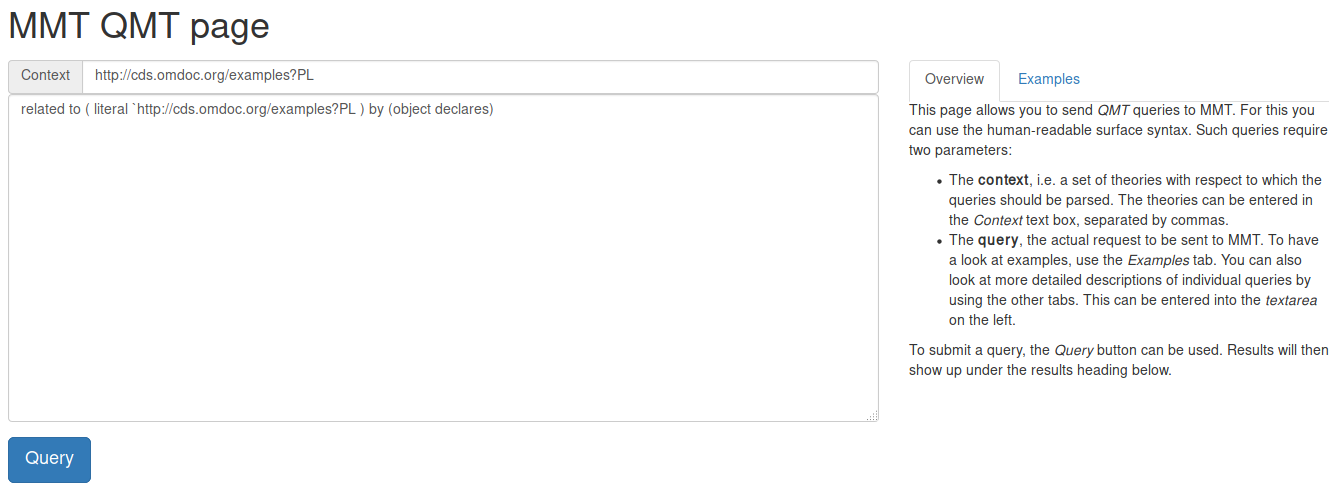
\includegraphics[width=1.0\textwidth]{imgs/QMTquery.png}
  \end{center}
  \caption{QMT Web Interface for entering Queries. }
  \label{fig:webinterface:entering}
\end{figure}

\begin{figure}[h]
  \begin{center}
    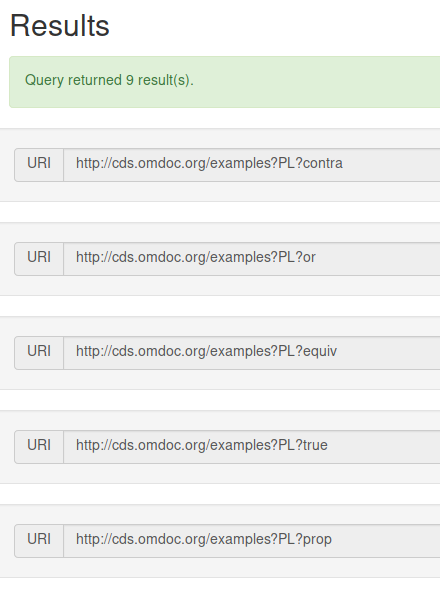
\includegraphics[width=0.5\textwidth]{imgs/QMTresults.png}
  \end{center}
  \caption{QMT Web Interface for displaying results. }
  \label{fig:webinterface:results}
\end{figure}

The web interface consists of two parts, an interface to enter queries as well as a result listing. 

The interface for entering queries can be seen in Figure~\ref{fig:webinterface:entering}. 
To submit a query, the user has to fill out two fields and click the \identifier{Query} button. 
The fields to be filled are the context and the query itself. 

As described previously, the context is a set of theories with respect to which the queries should be parsed. 
It can be entered in the \identifier{Context} text box separated by commas. 
The query, in surface syntax, can be entered in the main text area on the left. 

The display of results can be found in Figure~\ref{fig:webinterface:results}. 
On the web interface this is located below the entering interface and only shows up once results have been received. 
The interface is very plain and only shows two pieces of information, the number of results and each individual result. 

% Finish (eventually)
\newpage
% !TEX root = ../thesis.tex
\section{Conclusion}\label{sec:conclusion}

In this thesis, we have addressed the research question on how to connect different mathematical knowledge systems
in a generic, efficient and scalable manner to enable transparent, semantics-aware, distributed computation. 

To do this, we decided to make use of the Math-In-The-Middle paradigm. 
Using Virtual Theories, QMT and SCSCP we have created a solution that indeed provides a solution to this question. 
To achieve this we have had to address all three initial aspects. 

\begin{description}
  \item[A generic mechanism to manage and sync knowledge stored in MKS]\quad\\
    Using \lmfdb\ as an example, we have seen how to build a virtual theory layer acting as such a mechanism.  
    Our core contribution here is the choice of using Codecs to ensure separation of semantic and realized types. 
    This choice has turned out exactly right -- enabling our mechanism to easily integrate with different systems while at the same time not being ad-hoc. 
    This makes it different and better than existing approaches. 
    
  \item[A System-Independent Query Language]\quad\\
    We have furthermore built on top of the existing QMT language of the MMT system. 
    Instead of choosing to use a query language that relies on a specific data structure we can now see that we made the right choice here. 
    
    QMT was designed from the ground up to enable formulation of representation-independent queries. 
    Even though it required a refactoring and some extensions to properly deal with distributed computations, we have seen that this choice fits in well with the mechanism of codecs and almost naturally extends the knowledge representational aspects of the MiTM approach to computational ones. 
  
  \item[A Lower-Level Communication Layer] \quad\\
    For this layer, we choose to use the SCSCP protocol. 
    Along with the other two layers, and especially inside this one, we can see how it was a good choice to build on a system-independent framework. 
    The representation of objects using OpenMath or \omdocmmt\ terms enabled systems to easily expose their computational functionality. 
    This reaffirms again that communication between different specialist systems is possible without having to rely on an industry standard of having to rely on ad-hoc solutions -- a generic pattern like the one here is possible. 
\end{description}

To reflect on our contribution further, we take a final look at Jane's initial example of cross-system communication. 

\subsection{Revisiting the Use-Case For Cross-System Communication}\label{sec:conclusion:example}

With all the pieces in place, we can now see how our architectural choices help Jane express her computational problem in QMT. 

\begin{example}\label{example:cross}
  Jane's example expressed as a QMT Query. 
  \begin{lstlisting}[language=qmt]
  use "gap" for (
    use "lmfdb" for {*
      x in (
        related to ( literal `lmfdb:db/transitivegroups?group ) by (object declares)
      ) | holds x (
        x commutative x *=* true
      )
    *} 
  ) map x => cyclic x)
  \end{lstlisting}
\end{example}

% !TEX root = ../thesis.tex
\begin{figure}[h]
  \begin{center}
    \begin{tikzpicture}[xscale=7,yscale=3]\normalsize
      \node[draw] (s) at (0,0) {Sage};
      \node[draw] (m) at (1,0) {MMT};
      \node[draw] (g) at (2,0) {GAP};
      \node[draw] (l) at (1,-1) {LMFDB};
      \draw[->] (s) to[bend left=15] node[above] {\footnotesize 1: $Q@S$} (m);
      \draw[->] (m) to[bend left=15] node[right,near end] {\footnotesize 2: $Q'@L$} (l);
      \draw[<-] (m) to[bend right=15] node[left,near end] {\footnotesize 3: $34G@L$} (l);
      \draw[->] (m) to[bend left=15] node[above] {\footnotesize 4: $34G@G$} (g);
      \draw[<-] (m) to[bend right=15] node[below] {\footnotesize 5: [t,f,\ldots]} (g);
      \draw[<-] (s) to[bend right=15] node[below] {\footnotesize 6: [t,f,\ldots]} (m);
    \end{tikzpicture}
  \end{center}

  \caption[A MiTM use-case]{
    Elaborated technical details for Cross-System-Communication Use-Case. 
    Compare with Figure~\ref{fig:mitmcaseintro}. 
  }
  \label{fig:mitmcase}
\end{figure}
We can now also have another look at Figure~\ref{fig:mitmcaseintro}. 
In Figure~\ref{fig:mitmcase} the steps of this process are annotated with more technical details. 
\begin{enumerate}
  \item Jane formulates a QMT Query which expresses this hypothesis and sends it to \mmt. 
  This is the one shown above and consists of two parts. 
  The first part uses \lmfdb\ to retrieve all abelian (commutative) groups from \lmfdb. 
  This sub-query corresponds to Example~\ref{example:lmfdblong} and is in lines 2-8. 
  The second part uses GAP to check if a group is indeed cyclic. 
  Here, another \identifier{I()} query is used (line 1) to check if each of the results is indeed cyclic by using \identifier{map}. 
  
  \item \mmt\ identifies the inner \lmfdb\ query, translates and sends it to the \lmfdb API. 
  
  \item \mmt\ receives a list of $34$ results from \lmfdb\ and translates these back into Math-In-The-Middle terms. 
  
  \item \mmt\ then translates these intermediate results into objects that GAP can understand. 
  Next it translates the remainder of the query, and sends it to GAP along with the intermediate results using the SCSCP protocol. 
  
  \item GAP responds to the query and sends back a list of $34$ boolean (OpenMath) objects.
  This lists contains both \inlinecode{true} and \inlinecode{false}, because it turns out that the original hypothesis is false. 
  
  \item Finally, \mmt\ translates this set of results into a Sage objects which are then delivered back to Jane. 
\end{enumerate}

Most of these steps are hidden from Jane -- she only sends a single QMT Query. 
This makes this example truly a transparent, distributed cross-system communication. 

As we have seen the approach maintains object semantics across systems -- this is illustrated by Jane never seeing a $0$ or a $1$ which is stored inside of \lmfdb. 
Furthermore, she never knows that the abelian is stored in \lmfdb\ as the \identifier{ab} property -- no insight into \lmfdb\ is required. 

\subsection{Outlook}\label{sec:conclusion:outlook}

Currently, steps 1 - 5 in are implemented inside of \mmt\ and are fully functional. 
This once again shows that the MiTM approach is suitable of facilitating cross-system communication and was a valid choice. 
Furthermore, the approaches above are indeed feasible and improve on existing systems. 

However, work in this area is far from complete. 
Apart from extending the approach to include more systems and testing it in more settings, 
there are a several improvements that can be made. 

Consider for example QMT. 
Currently, sub-queries need manual annotation to mark them as being used with external systems. 
During this thesis it has been speculated that an automatic approach intercepting each intermediate result would be to computationally expensive. 
In a future extension of the query language, one might instead consider analyzing the structure of each query and automatically annotating parts of the query to be evaluated with different systems. 

Furthermore, as stated above, step 6 of the example has not yet been implemented. 
This means making QMT available to the Sage system.
Thus we need to implement one of two approaches, either make a Sage specific API, or exposing the QMT interface via SCSCP and building a client inside of Sage. 
The latter of these options seems appealing, and has been hinted on during this thesis. 
However, this approach requires more thought than might initially seem necessary. 

It is straightforward to send queries from Sage, however it is not as easy to receive the results. 
As stated above, these need to be translated into something that Sage specific. 
Hence, when posing the Query, \mmt\ needs to be made aware that the Query is coming from Sage. 
To implement this in a generic fashion that can eventually be extended to systems beyond the ones mentioned here, one could either add a separate case to the query language, or build this into an argument to be passed only via SCSCP. 
  
\subsection{Acknowledgements}\label{sec:conclusion:outlook:acknowledgements}

The author acknowledges that the work for this project has been financially supported by the OpenDreamKit Horizon 2020 European Research Infrastructures project (\#676541). 
Furthermore, the author expresses his thanks to John Cremona for his help on understanding the structure of objects inside of \lmfdb\ as well as all members of the KWARC group, and in particular Michael Kohlhase, for their input and help during the design and implementation phases of the work described here. 

\newpage
\printbibliography

\newpage
% !TEX root = ../thesis.tex
\appendix
\section{Detailed Contributions And Acknowledgements}\label{sec:contrib}

I give a short overview of which parts of the work described in this thesis have been created only by me, and which have been created collaboratively together with others. 
This has already been acknowledged with citations. 

\paragraph*{Section~\ref{sec:intro}}
The preliminaries, like the \omdocmmt\ infrastructure, the OpenDreamKit project, and the Math-In-The-Middle approach, have each been worked on collaboratively with others. 
In particular, Figure~\ref{fig:classicalconnect}, Figure~\ref{fig:mitmconnect}, as well as the example presented in Figure~\ref{fig:mitmcaseintro} have been adapted from different OpenDreamKit project papers, written collaboratively with other project members. 
The research question, as well as the extensions to the QMT Query Language, have been contributed by myself for the use within this thesis. 

\paragraph*{Section~\ref{sec:mmt}}
In this section I detail backgroud information about the \mmt\ system, especially for readers not familiar with it. 
The \mmt\ system, and the \omdocmmt\ infrastructure, as indicated, was developed within the KWARC group, however this section has been written from the ground up by me. 
It re-uses a frequent example from within the research group; Figure~\ref{fig:theorygraph} is an adapted version of a previously existing Figure. 

\paragraph*{Section~\ref{sec:mitm}}
In this section, I related the Math-In-The-Middle approach to the research question. 
The Math-In-The-Middle approach itself was not invented by me, it been designed together with other members of the OpenDreamKit project. 
Figure~\ref{fig:mitmontology} is a customized version of a Figure that has appeared in different OpenDreamKit project presentations. 
The SCSCP protocol existed prior to the OpenDreamKit project, and has been originally designed by others. 
Within the scope of this thesis, I have implemented the protocol within \mmt\ along with a pure OpenMath implementation on my own.  

\paragraph*{Section~\ref{sec:vt}}
In this section, I describe the structure of \lmfdb\ and describe the implementation of Virtual Theories. 
\lmfdb\ is a database that is maintained by others, and as such I do not claim to have developed the structure, or found the knowledge contained within it. 
The codec and virtual theory infrastructure described here has again been developed collaboratively in the KWARC group; some parts of the implementation have been written by others. 
All Figures within this Section are my own. 

\paragraph*{Section~\ref{sec:qmt}}
In this section, I describe the QMT Query Language, and a few syntax extensions. 
The language itself, and the basic implementation for concrete theories, has been developed by the KWARC group, and in particular Florian Rabe. 

\paragraph*{Section~\ref{sec:comm}}
In this section I describe my extensions to the QMT Query Language. 
These include evaluation within Virtual Theories, the syntax on the MMT surface level, and the web interface. 
I have developed and implemented these, and as such all Figures and Screenshots in this Section are my own. 

\paragraph*{Section~\ref{sec:conclusion}}
In this section I revisit the collaboratively developed use-case, and then give an outlook and a conclusion. 
Figure~\ref{fig:mitmcase} is again heavily adapted from an OpenDreamKit presentation, all other text and Figures are my own. 

\end{document}
